\documentclass[openright,twoside,a4paper,english,12pt]{report}

%% ==========================
%% Template adapted to the School of Biological Sciences need
%% main LaTeX set up for a Geology and Geophysics thesis keeps evolving into unknown yet funky beasties. I borrowed this set-up from Kathryn Hardacre who got it from 
%% Jon Perry. Undoubtedly, I will add some extras as well


\usepackage{edthesis}
\usepackage{fancyhdr}% Use titlesec to put Chapter title on right
\usepackage{babel}
\usepackage{a4}
%\usepackage{sectsty}
\usepackage[round]{natbib}
\usepackage{amsfonts}
\usepackage{amsthm}
\usepackage{eucal}
\usepackage[intlimits]{amsmath}
\usepackage{graphicx}
\usepackage{lscape}
\usepackage{longtable}
\usepackage{rotating}
%\usepackage{supertabular}
%\usepackage{nomencl}
\usepackage[percent]{overpic}
%\usepackage{tocbibind}
\usepackage{caption}
\usepackage{pdfpages}
\usepackage{glossaries}
\usepackage[utf8x]{inputenc}

%% some handy macros
\setlength{\headheight}{15pt}

\makeglossary
\newcommand{\pd}{\partial}
\renewcommand{\vec}{\boldsymbol}
\DeclareMathOperator{\Ber}{Ber}
\DeclareMathOperator{\Bei}{Bei}
\DeclareMathOperator{\Ker}{Ker}
\DeclareMathOperator{\Kei}{Kei}
\DeclareMathOperator{\integer}{int}
\DeclareMathOperator{\floor}{floor}
\DeclareMathOperator{\var}{var}
\DeclareMathOperator{\const}{constant}
\DeclareMathOperator{\maxval}{max}
%\bibliographystyle{plainnat}
\bibliographystyle{jmb}

% change font for captions
\renewcommand{\captionfont}{\sffamily}
\renewcommand{\captionlabelfont}{\bf}

% change font for chapter/section headings
%\allsectionsfont{\sffamily}

% funky graphics + text in lr bottom
\begingroup% 
\ifx\MakeISMBox\undefined%
\gdef\MakeISMBox#1#2#3{%
  \begin{overpic}[width=#1]{#2}%
    %\put(0,0){\includegraphics[width=#1]{#2}}%
    \put(98,2){\makebox(0,0)[br]{#3}}%
  \end{overpic}}%
\fi\endgroup%

% workaround for color in ed_thesis
\begingroup% 
\ifx\color\undefined%
\gdef\color[#1]#2{}%
\fi\endgroup%

% workaround for href in ed_thesis
\begingroup% 
\ifx\href\undefined%
\gdef\href#1#2{#2}%
\fi\endgroup%

% defining units for nomenclature packages
\newcommand{\nomunit}[1]{%
%  \renewcommand{\nomentryend}{\hspace*{\fill}[#1]}%
}

% Alternative style of head and foot
\pagestyle{fancy}% Used when using fancyhdr.sty
\renewcommand{\headrulewidth}{0.4pt}
\renewcommand{\footrulewidth}{0pt}
\renewcommand{\chaptermark}[1]{%
 \markboth{\MakeUppercase{%
 \chaptername} \ \thechapter.%
 \ #1}{}}
\renewcommand{\sectionmark}[1]{%
 \markright{ \ \thesection%
 \ #1}{}}

%\rhead{\thepage}
\fancyhead[LE,RO]{\thepage}
\fancyhead[LO]{\sl \leftmark}
\fancyhead[RE]{\sl \rightmark}
\fancyfoot{}

%Tidy up hyphenations as best as possible
\pretolerance = 600 % covers most paragraphs
\tolerance = 7000 % covers the nasty cases

%Tidy up hanging sentences as best as possible
\widowpenalty=10000

% To get the correct margins for the regulations for psglg1 and psglg3
\setlength{\oddsidemargin}{1.35cm} %margins set up for psglg1
\setlength{\evensidemargin}{-0.1cm}
\setlength{\topmargin}{0cm}
\setlength{\textwidth}{14.55cm}
\setlength{\textheight}{22.3cm}


\newdimen\tablewd
\newdimen\tablewidth
\newdimen\captionwd
\newbox\tempbox
\newskip\tableleftskip%
\newskip\tablerightskip%
\newskip\tablecapleftskip%
\newskip\tablecaprightskip%
\newskip\tablefootleftskip%
\newskip\tablefootrightskip%

\def\toprule{\noalign{\ifnum0=`}\fi
  \hrule \@height .5\p@
  \hrule \@height 6\p@ \@width \z@
  \futurelet \@tempa\@xhline}

\def\colrule{\noalign{\ifnum0=`}\fi
  \hrule \@height 3.5\p@ \@width \z@
  \hrule \@height .5\p@
  \hrule \@height 5\p@ \@width\z@
  \futurelet \@tempa\@xhline}

\def\botrule{\noalign{\ifnum0=`}\fi
  \hrule \@height 3.25\p@ \@width \z@
  \hrule \@height .5\p@
  \hrule \@height 3.25\p@ \@width\z@
  \futurelet \@tempa\@xhline}
\long\def\tableparts#1#2#3{%%%%%%%%%%%%%%%%%%%%%%%%%%%%% #1-caption #2-body #3-footnote
    \setbox\tempbox\vbox{#1}                          %% to calculate width caption
    \addtocounter{table}{-1}                          %%
    \settowidth{\global\tablewd}{\tablebodyfont#2}    %% \captionwd - caption of width
    \tablewidth\hsize                                 %% \tablewd   - table width
    \advance\tablewidth-\tablewd
    \divide\tablewidth 2
    \global\tableleftskip\tablewidth
    \global\tablerightskip\tablewidth
    \ifdim\captionwd>\hsize
        \global\tablecapleftskip\tablewidth
        \global\tablecaprightskip\tablewidth %plus2fill
    \else
        \global\tablecapleftskip\tablewidth  %plus2fill
        \global\tablecaprightskip\tablewidth %plus2fill
    \fi
    \global\tablefootleftskip\tablewidth
    \global\tablefootrightskip\tablewidth %plus2fill
    {#1 \par}%
    {\tablebodyfont #2\par}%
    {\tablefootfont #3\par}%
}

\def\tablebodyfont{\fontfamily{\rmdefault}\fontsize{8}{9}\selectfont\leftskip\tableleftskip\rightskip\tablerightskip}
\def\tablefootfont{\fontfamily{\rmdefault}\fontsize{7}{9}\selectfont\leftskip\tablefootleftskip \rightskip\tablefootrightskip}



%========================= ALTERATIONS ========================= 

%Paragraphs
\setlength{\parindent}{0em}
\setlength{\parskip}{\baselineskip}

%Alternative methods
%\lefthyphenmin=63
%\righthyphenmin=63
%\hyphenpenalty=10000

%To introduce 1.5 spacing
\renewcommand{\baselinestretch}{1.5}

\begin{document}
\newboolean{edthesis}
\setboolean{edthesis}{true}
%\setboolean{edthesis}{false}

\newcommand{\dir}{../preface}

%========================= PREFACE ========================= 
\ifthenelse{\boolean{edthesis}}
{  \begin{prefacepart}
   \pagenumbering{roman} 
}
{
  \frontmatter
}

\ifthenelse{\boolean{edthesis}}{\begin{singlespace}}
\thispagestyle{empty}

\begin{minipage}{\textwidth}
\end{minipage}
\begin{center}
\vspace{2cm}
{ \Huge Modular Cell-free systems and their adaptable logic as core processing machinery}
  \par
  \vspace{1cm} 
{\Large Felipe A. Millacura \par}

\end{center}
\vfill
\begin{center}
\vspace{5cm}    
\centerline{
\includegraphics[width=0.5\textwidth]{../preface/UoECentredLogoCMYKv1160215.png}}
\vspace{0.5cm}
Thesis submitted in fulfillment of\\
the requirements for the degree of\\ 
Doctor of Philosophy\\
University of Edinburgh \\
2020
\end{center}

\newpage
\thispagestyle{empty}

\ifthenelse{\boolean{edthesis}}{\end{singlespace}{}


\chapter{Declaration}
\vspace*{2\baselineskip}
 I declare that this thesis has been composed solely by myself and that it has not been submitted, in whole or in part, in any previous application for a degree. Except where states otherwise by reference or acknowledgment, the work presented is entirely my own.
\vspace{6\baselineskip}\\
\begin{flushright}
\hspace*{\fill}
Felipe Aguilera Millacura
\newline
January 2021
\end{flushright}


\cleardoublepage

\chapter{Abstract}
\markboth{\MakeUppercase{Abstract}}{\MakeUppercase{Abstract}}
While Synthetic Biology represents a promising approach to solve real-world problems, 
the use of genetically modified organisms (GMO) is still a cause of legal and environmental concerns. 
Cell-free systems (CFS) are an emerging technology where cell extracts are used instead of genetically-modified cells, 
thus, not presenting a "living prospect" applicable to current legal regulations.

Since there is a need for development of novel systems using the cell-free approach, and considering that most attempts have
been focused on mimicking normal cell behaviour. This work has as principal aim to generate modular cell-free and cell-based 
systems capable of not only detect variables present in the environment, such as heavy metals or antibiotics, but also analyse
 them via the usage of unnatural behaviours, such as logic gates.

In vivo logic gates, for instance, have proven difficult to combine into larger devices. 
Here it is explained a cell-based logic system, ParAlleL, which decomposes a large genetic circuit 
into a collection of small subcircuits working in parallel, responding each subcircuit to a different combination of inputs. 
A final global output is then generated by a combination of the responses. Using ParAlleL, for the first time a completely
functional 3-bit full adder and full subtractor were generated using \textit{Escherichia coli} cells, as well as a calculator-like
display that shows a numeric result, from 0 to 7, when the proper 3 bit binary input is introduced into the system. 
This parallel approach facilitates the design of cell-based logic gates by the decomposition of complex processes into their main
components, avoiding the need for complex genetic engineering and solving some legal limitations.

Cell-free systems, on the other hand, have emerged as a possible solution but much work is needed to optimize their functionality 
and simplify their usage for Synthetic Biology. Here it is presented a transcription-only genetic circuit (TXO), which is independent
of translation or post-translation maturation. RNA aptamers are used as reaction output allowing the generation of fast, reliable and
simple-to-design transcriptional units. TXO cell-free reactions and their possible applications become a promising new tool for fast
and simple bench-to-market genetic circuit and biosensor applications.

Additionally, it's shown a versatile cell-free system based on the master survivalist bacteria \textit{Cupriavidus  metallidurans} CH34,
able of not only sensing environmental variables, such as heavy metals, but also synthesize proteins and produce bioplastics. This novel 
cell-free  chassis  comes after the discovery of the unstable genome that this bacteria carries, which is also explained here, offering 
novel possibilities of development considering the cell free approach.
\chapter{Lay Summary}
\markboth{\MakeUppercase{Lay Abstract}}{\MakeUppercase{Lay Abstract}}
In an era where Genetically Modified Organisms (GMOs) are a mainstream topic within society, a necessity for different approaches without the usage of living organisms is needed. One of the most promising technologies is the use of Cell-free systems which doesn't imply a living prospect applicable to current legal or moral society restrictions.

During Cell-free preparation the cell wall is ripped off, the insides collected, and the cell catalyst used to produce new kinds of molecules and biological processes without the evolutionary constraints of using intact living cells.

In this work a novel cell-free system approach that allows the detection of toxic pollutants, such as heavy metals, and also able to analyse mixed samples as real environmental samples commonly carrying more than just one contaminant is presented. 

Simple biological molecules such as RNA are used in our system to accelerate the detection process, allowing us to use different approaches rather than imitating ordinary cell conduct, which is the most common scientific rationale to approach these kind of problems.
\chapter{Acknowledgements}
%\usepackage[pages=some]{background}
%\backgroundsetup{
%contents={%
 % \includegraphics[width=\textwidth,height=\textheight]{example-image}
%  }%
%}
\markboth{\MakeUppercase{Acknowledgements}}{\MakeUppercase{Acknowledgements}}
Firstly, I would like to express my sincere gratitude to my supervisor Prof. Christopher E. French for the continuous support of my PhD research, for his patience, motivation, and immense knowledge. I could not have imagined having a better supervisor and mentor for my PhD study, as his guidance helped me performing the research and writing of this thesis.
My sincere thanks to Dr. Rojas and Dr. Janssen. It would not be possible to be here writing this thesis without the opportunity given to join their respective research teams, enlightening me during my first glances in research.
I thank my fellow labmates for the stimulating discussions, their constant support and encouragement and for all the fun we have had during the last four years. A special thanks to Alejandro, Chao-Kuo, Jan, Marcos, Prabu, Antreas, Dariusz, Paulina, Christopher, Eric, Florentina and Mengxi who helped me during different stages of my PhD. A special recognition to all master and undergraduate students formed in our lab, who motivated me with their enthusiasm and even sometimes silly questions. Thanks to Bethan, Konstantinos, Gedis, Athan, Franklin, Brendan, Teri, Niels, Alexander, Cal, Nuoya, Juro, Jovanna and Stefano. 
To my ELE-EAP mates and instructors: Yermek, Nurlan, Daniyar, Korlan, Mohammed, Dayoung, Dauren, Soyoung, Ainur, Kuanish, Bakyt, Aigerim, Philip, Peter and Barbara. And also to the CodeClan mates: Dhileas, Jennie, Rhiannon, Ric, Kostas, Jonathan, Kuba, Miles, David, Stephanie, Del, Aileen, and Mhairi.
Most importantly, I would like to thank my family for the unconditional support. To Griselda and Francisco who are my major motivation to succeed in life. To my dad and cousins who convinced me to visit Chile while doing my PhD. Specially to Camila and Cassandra. To my aunts and uncles for the love given. To all my friends who even though the distance always tried to keep in touch, an honorific mention to Valeska, Ariel and Cristian for their incredible support. Thanks also to Macarena, Leyla and Merari who kept me rational and sane during the harsh times. Finally, thanks to Maria Victoria who always believed in me even more than what I did myself. Thanks to all of you I am able to finish this PhD thesis and, hence, this is also part of your success. Your support and patience contributed to make the impossible possible.

This research would not be feasible without the support of the 'Agencia Nacional de Investigacion y Desarrollo (ANID, formerly CONICYT)' and its program 'Formación de Capital Humano Avanzado' who made me a beneficiary of the 'Becas Chile-PhD 72170403'.
\chapter{Agradecimientos}
%\usepackage[pages=some]{background}
%\backgroundsetup{
%contents={%
 % \includegraphics[width=\textwidth,height=\textheight]{example-image}
%  }%
%}
\addtolength{\topmargin}{-.875in}
\addtolength{\textheight}{1.75in}
\markboth{\MakeUppercase{Agradecimientos}}{\MakeUppercase{Agradecimientos}}
Primero, me gustaría expresar mi sincera gratitud a mi supervisor, el Prof. Christopher E. French por el continuo apoyo otorgado durante mis estudios de PhD, por su paciencia, motivación e inmenso conocimiento. No habría poder tenido un mejor supervisor y mentor para mis estudios Doctorales, ya que su guía me ayudo a realizar la investigación y el escrito de esta tesis.
Mis sinceros agradecimientos al Dr. Rojas y el Dr. Janssen. No podría ser posible el estar escribiendo esta tesis sin la oportunidad que me entregaron al permitirme formar parte de sus respectivos equipos de investigación, iluminándome durante mis primeros pasos.
Agradezco a mis compañeros de laboratorio por las estimulantes conversaciones, su constante apoyo y palabras de aliento, y por toda la diversión que tuvimos durante los últimos cuatro años. Un agradecimiento especial a Alejandro, Chao-Kuo, Jan, Marcos, Prabu, Antreas, Dariusz, Paulina, Christopher, Eric, Florentina y Mengxi quienes me ayudaron durante diferentes etapas de mi PhD. Un reconocimiento especial a todos los estudiantes de maestría y pregrado formados en nuestro laboratorio, quienes me motivaron con su entusiasmo e incluso con algunas preguntas tontas. Gracias a Bethan, Konstantinos, Gedis, Athan, Franklin, Brendan, Teri, Niels, Alexander, Cal, Nuoya, Juro, Jovanna y Stefano. 
A mis compañeros e instructores del ELE-EAP: Yermek, Nurlan, Daniyar, Korlan, Mohammed, Dayoung, Dauren, Soyoung, Ainur, Kuanish, Bakyt, Aigerim, Philip, Peter y Barbara. También a mis compañeros de CodeClan: Dhileas, Jennie, Rhiannon, Ric, Kostas, Jonathan, Kuba, Miles, David, Stephanie, Del, Aileen, y Mhairi.
Me gustaría agradecer a mi familia por su apoyo incondicional. A Griselda y Francisco por ser mi mayor motivación para salir adelante en la vida. A mi padre y primos quienes me convencieron en visitar Chile mientras realizaba mi PhD. Especialmente a Camila y Cassandra. A mis tías y tíos por el cariño entregado. A todos mis amigos, que aun a la distancia trataron siempre de mantener el contacto, una mención honorifica a Valeska, Ariel y Cristian por su increíble apoyo. Gracias también a Macarena, Leyla y Merari quienes me mantuvieron racional y cuerdo durante los tiempos difíciles. Finalmente, gracias a María Victoria quien creyó siempre en mi incluso más de lo que yo mismo hacía. Gracias a todos ustedes hoy soy capaz de terminar esta tesis, y por lo tanto, esta victoria también es suya. Vuestro apoyo y paciencia contribuyó a hacer lo imposible posible.
Esta investigación no seria factible sin el apoyo de la 'Agencia Nacional de Investigación y Desarrollo (ANID, ex CONICYT)' y su programa 'Formación de Capital Humano Avanzado' quienes me hicieron benefactor de la 'Beca Chile-PhD 72170403'.

{\setlength{\parskip}{0ex plus 0.5ex minus 0.2ex}
\ifthenelse{\boolean{edthesis}}
 {
  \begin{singlespace}
 {}
\tableofcontents
\listoftables
\listoffigures

% Glossary stuff
%\chapter{Glossary}
%\makeglossaries
%\newacronym{gcd}{GCD}{Greatest Common Divisor}
 
%\newacronym{lcm}{LCM}{Least Common Multiple}
 

Given a set of numbers, there are elementary methods to compute 
its \acrlong{gcd}, which is abbreviated \acrshort{gcd}. This process 
is similar to that used for the \acrfull{lcm}.
 
%\clearpage
 
%\printglossary[type=\acronymtype]

\cleardoublepage
%\renewcommand{\nomname}{List of Symbols}
%\markboth{\MakeUppercase{\nomname}}{\MakeUppercase{\nomname}}
%\addcontentsline{toc}{chapter}{List of Symbols}
%\printglossary
\ifthenelse{\boolean{edthesis}}
 {
  \end{singlespace}
 }{}
}

\ifthenelse{\boolean{edthesis}}
{
   \end{prefacepart}
   \pagenumbering{arabic} 
}
{\mainmatter}
%========================= CHAPTERS ========================= 
\renewcommand{\dir}{../introduction/chapter/}
\chapter{General Overview}

Since the beginning of time life has made his way through multiple adverse conditions. Organisms have evolved from single cells interacting directly with their environment, to specialised multi cellular entities that respond specifically to different stimuli. Even though cells can specialise their functions by differentiating into diverse cell types, aggregating into tissues or organs, or by generating a variety of organisms, they all respond to the same paradigm. DNA is used to save and protect the hereditary information, which is later transcribed into functional orders in the form of RNA, being most of the time later translated into protein products that execute those final orders. 
This process was broadly studied on the twentieth century in order to explain how life works.
DNA was discovered to be the source of information that carries and saves all instructions for securing life mantainance over generations (\cite{watson1953molecular}). Although RNA and protein synthesis can occur almost simultaneously in the cell  (\cite{miller1970visualization}), proteins need to acquire their secondary, tertiary or quaternary structure to become functional, with even sometimes needing post-translational modifications to work.  


One of the first mentions of Synthetic Biology can be tracked way back to \cite{leduc1912biologie}, who sought to synthesise life "by directing the physical forces which are its cause".


Cell-free expression systems are a powerful tool in applications where cell based expression systems are
too variable, slow, difficult to store or prohibitive due to legislation on the release of genetically modified
organisms. Cell-free systems (CFS) are not without their limitations; since their very nature is to be a defined,
precisely controlled system that lacks self-replicating functionality, they depend on a limited quantity of
supplies, such as ATP, amino acids and nucleotides \cite{kwon2015high}. Consequently, in-vitro
synthesis of protein is limited by two dimensions: the overall maximum protein amount that can be
synthesized with the supplied components, and the time during which the CFS stays active before
background processes and chemical deterioration have used up supplies or inactivated the system \cite{carlson2012cell,bernhard2013cell,kwon2015high} 
One of the most promising applications of CFS is the possibility to design cell-free biosensors, which do not
present a living prospect subject to the current GMO legal regulations and offer an alternative to standard
analytical techniques, such as ICP-MS and ICP-OES. However, cell-free biosensors that rely on protein
expression also present the
common limitations of CFS, such as a long response time and a lack of
precursor regeneration. Sensors that could function without the need for protein expression would drastically
reduce the requirements for such a system. Paige et al., (2011) designed synthetic fluorescent RNA
aptamers that mimic fluorescent proteins without the need for translation. The secondary structure of these
aptamers presents a loop in which a fluorophore is trapped, conferring the same intramolecular
immobilization that confers fluorescence in fluorescent proteins (Paige et al. 2011; Strack et al. 2013).
These RNA aptamers also suffer from several limitations as incorrect folding is observed under non optimal
thermal or ionic conditions (Autour et al. 2016). Improved aptamers with a stronger secondary structure,
such as Broccoli and iSpinach, show increased stability under non-optimal conditions (Filonov et al. 2014,
Autour et al. 2016). Both aptamers are based on the 95 base core sequence of Spinach2 and can be flanked
by a tRNA scaffold, increasing the stability of their secondary structures (Filonov et al. 2014, Autour et al.
2016, Strack et al. 2013). However, these were designed for in vivo use (e.g. analysing RNA quantities) and
have never been tested as outputs for a cell-free sensor. Such a sensor could require only transcription, not
translation, hence could be much faster and simpler.
On the other hand, the simplicity of CFS can become a disadvantage when complex processes need to beperformed. For instance, the high dependence on E. coli as a model organism generates a problem, since
genes or genetic pathways from non-model organisms or obtained by metagenomic studies, may fail to be
expressed in standard organisms. Moore et al., (2016 and 2017) have attempted to solve this issue by using
non-model bacteria, such as Bacillus or Streptomyces, for the generation of new cell-free TX/TL systems.
This approach can be applied to other organisms, such as extremophiles, in order to use their unique
capacities. For example, Cupriavidus metallidurans possesses the capability to tolerate, remove and
degrade diverse environmental pollutants(Millacura et al., 2017). A cell-free system based on Cupriavidus
metallidurans
extract might show increased tolerance for heavy metals and might be superior for heavy
metal sensors.
Another challenge for CFS is to analyze multiple variables simultaneously. As they rely on the normal cell
processing/synthesis machinery (interaction between transcription factors, polymerases, ribosomes, and
other diverse macromolecules), they suffer the same issues as a living organism. Furthermore, when
complex interactions are carried out, problems may arise due to kinetic mismatches, lack of oscillation or
Boolean/Reversible designs (Guz et al., 2016). The generation of cell-free systems that respond to variables
using totally synthetic processing machinery seems to be one of the most promising approaches. There
have been some attempts to generate logic gates without mimicking normal cell machinery (Bordoy et al.,
2016, Chatterje et al., 2016, Kim et al., 2014 and Zhang et al., 2016), however, due to their dependence on
translation and/or the need for manually addition of foreign oligonucleotides (Kim et al., 2014) they still show
slow response. Additionally, some of them rely on recombination processes that make their implementation
even more complicated than under in vivo conditions (Zhang et al., 2016).
In electronics, a single circuit accepts one or more binary inputs to generate one or more binary outputs.
There have been many attempts to replicate such circuits using in vivo genetic networks. A typical biological
logic gate consists of an output macromolecule that is produced only if the corresponding pattern of inputs is
present, inputs that are commonly associated with the presence of transcriptional regulators, transcription
factors, polymerases or other macromolecules \cite{silva2008mining} . Here we propose an
alternative approach, BioLogic, which decomposes a large circuit into a collection of small subcircuits,
solved in parallel. Rather than having a single type of cell (or genetic material) doing the computation, we
have separate versions (subcircuits) each reacting to a different combination of inputs and generating the
desired response by combination of each final output. For instance, if each input bit is considered in two
forms, ZERO and ONE, each of which is essential to certain output agents, any arbitrary pattern of outputsfor any pattern of inputs could be generated, making all kinds of binary operation possible
A further proposal is to achieve this goal by using just a transcriptional genetic network, without need for
translation. Each agent in this case, rather than a cell, is a plasmid or double stranded DNA that does not
possess functional transcriptional networks (Figure 1). As cell-free systems can assemble DNA parts in vitro
at very low cost by using cell extracts instead of enzyme cocktails (Casini et al., 2015), and Golden Gate
Assembly is an excellent tool to assemble multiple DNA fragments in a defined linear order, by using type
IIS restriction enzymes (Engler et al., 2008), these techniques may be combined to generate a new and
inexpensive in vitro system, which through DNA assembly and processing (hereafter DNALogic) would be
able to sidestep common problems associated with the use of live cell based systems. As a "triggering" step
is vital for the DNALogic processing machinery, the novel CRISPR/Cpf1 technology (or similar) will be used
to generate the respective recognition and cutting steps. CRISPR/Cpf1 generates 5' overhanging cuts,
producing 8 nt sticky ends and cleaving at the 14th base from the PAM site TTN (Lei et al., 2017 and Li et al.,
2016). Due to its similarities to Type IIS restriction enzymes, Cpf1 can also be used to generate a new kind
of Golden Gate Assembly, which would not rely on the presence or absence of cutting sites, but on gRNA.
The gRNA expression system can be combined with the recognition step, working as a transduction system
between the detection and processing steps (Figure 1a).
This CRISPR triggered sequence recognition,
followed by cutting and ligation steps, would result not only in a fully functional transcriptional unit, but also in
a different double stranded genetic sequence, accomplishing the parameters for synthetic memory
generation explained and demonstrated in vivo by Siuti et al. (2013). This creates DNA memory that can not
only be later amplified and processed by sequencing and/or PCR (later response), but that can also
generate RNA expression of a fluorescent aptamer or a further gRNA if there is formation of a proper
transcription unit (immediate response).Figure 1. Proposed DNALogic system. A) crRNA expression is regulated by inducible promoters B)
Ribonucleoprotein formation is followed by recognition and cutting of the target DNA C) Ligation of the
overhangs produced by the Ribonucleoprotein generates a transcriptional unit D) Expression of the
transcriptional unit generates a functional fluorescent RNA aptamer.Aims:
This work has as its general aim the generation of a modular cell-free system capable of not only sensing
variables present in the surrounding environment, such as heavy metals, but that is also able of analyzing
them by using a totally synthetic in vitro logic gate.
Specific aims are:
1. Testing fluorescent RNA aptamers as output signals for cell-free sensors.
2. Developing Cpf1-based signal processing technology for use in cell-free systems.
3. Creation of an adaptable DNALogic gate, which allows memory and more complex analysis in cell free
systems.
4. Testing Cupriavidus metallidurans extracts as basis for metal-sensing cell free systems using
endogenous and exogenous metal sensing promoters.
5. Integrating these to develop a modular cell-free sensing system with versatile in-vitro signal processing.

\renewcommand{\dir}{../chapter1/chapter/}
\chapter{ParAlleL: A Novel Population-Based Approach to Biological Logic Gates}

\section{\textbf{Abstract }}

In vivo logic gates have proven difficult to combine into larger devices. 
Our cell-based logic system, ParAlleL, decomposes a large circuit into a collection of small subcircuits working in parallel,
each subcircuit responding to a different combination of inputs. 
A final global output is then generated by a combination of the responses. 
Using ParAlleL, for the first time a completely functional 3-bit full adder and full subtractor were generated using 
\textit{Escherichia coli} cells, as well as a calculator-style display that shows a numeric result, 
from 0 to 7, when the proper 3 bit binary inputs are introduced into the system. 
ParAlleL demonstrates the use of a parallel approach for the design of cell-based logic gates that facilitates 
the generation and analysis of complex processes, without the need for complex genetic engineering.

\section{\textbf{Introduction }}

A major challenge in the field of synthetic biology is the construction of complex logic circuits that analyze variables as in electronics; where a single circuit accepts one or more binary inputs to generate one or more binary outputs. A cell-based logic network consists of engineered cells producing an output macromolecule only if the corresponding pattern of inputs is present. The mechanism of analysis is commonly based on the use of transcriptional regulators, transcription factors, polymerases, receptors, or recombinases \cite{brenner2018synthetic}. Some examples of genetic circuits mimicking computational behavior are toggle switches, oscillators, boolean logic gates, feedback controllers, and multiplexers. Although there are genetic circuits that simulate computational behavior, the complex engineering of their biological chassis is affected by gene expression noise, mutation, cell death, undefined, and changing extracellular environments and improper interactions with the cellular context \cite{andrianantoandro2006synthetic}. Furthermore, complex genetic engineering is necessary when multiple input variables are analyzed, limiting the processing capacity of the system.

Biological multiplexers analyze one or more signals over a common transmission line using interconnected transcription factors, recombinases, antisense RNA, or CRISPR-like technology \cite{nielsen2014multi,roquet2016synthetic,brenner2018synthetic}. However, complex genetic engineering is needed for wiring the basic computational units, becoming inefficient for moving beyond simple NOT or AND logic gates or for scaling to 3 bit logic circuits. The complexity of the genetic engineering required can be reduced by using distributed logic circuits, where the computation is distributed among several physically separated cellular consortia that each sense only one signal and respond by secreting a communication molecule \cite{regot2011distributed}. As a circuit responds to one signal, but not another, due to spatial distribution, a change in the state of the system can be triggered as response, making synthetic learning possible \cite{macia2017synthetic,shipman2017crispr}. Even though the consortium approach makes Boolean circuit design simpler, it still shows a slow response and considerable complexity since each cell needs to recognize, synthesize and secrete a wiring molecule \cite{macia2016implementation}.

Here we propose an alternative logic architecture, which decomposes a large circuit into a collection of small subcircuits acting in parallel (hereafter ParAlleL). Rather than having a single type of agent (such as a genetically engineered cell) doing the computation, ParAlleL has separate types of agent that each react to a different combination of inputs. A final output is then generated by combination of the responses, making all kinds of binary operation possible. As an example, here we show the implementation of this concept using cells resistant to different combinations of antibiotics, with the response indicated by growth. This is used to demonstrate a completely functional 3 bit full adder and full subtractor, as well as a calculator-style display that shows digits from 0 to 7 based on three binary input bits.

\section{\textbf{Methodology }}

\subsection{\textbf{Reagents and Stock Solution Preparations}}

Antibiotic stock solutions were prepared as follows: 100 mg/ml carbenicilin disodium salt (Sigma-Aldrich \#C1389), 50 mg/ml kanamycin sulfate (PanReac Applichem \#A1493), 20 mg/ml chloramphenicol (Acros Organics \#22792), 10 mg/ml tetracycline hydrochloryde (Duchefa Biochemie \#T0150), 10 mg/ml gentamicin sulfate (Melford \#G0124), and 50 mg/ml spectinomycin.HCl (LKT Labs \#S6018). Developing solution contained 0.1 \%w/v bromothymol blue (Sigma-Aldrich \#114421) and 400 mM Trizma base pH7.5 (Sigma-Aldrich \#T1503).

\subsection{\textbf{Generation of Subcircuit Cells}}

\textit{E. coli} JM109 was transformed with 200–300 pg of plasmid pSB4A5 (AmpR) or pSB4C5 (ChlR) (Registry of Standard Biological Parts) and selected on 100 μg/ml carbenicilin (Am) or 20 μg/ml chloramphenicol (Ch), respectively. Cells carrying the first bit plasmid were made chemically competent \cite{chung1989one} and transformed with 200–300 pg of the 2nd bit plasmid, pSB1T3 (TetR) or pSB1K3 (KanR) (Registry of Standard Biological Parts). Selection was performed with the first antibiotic (Am or Ch) and the addition of 10 μg/ml Tetracycline (Tc) or 50 μg/ml kanamycin (Km), obtaining the two-bit combinations Km/Am (KA), Tc/Am (TA), Km/Ch (KC), and Tc/Ch (TC). This set of strains is sufficient to implement all two-bit binary operations.

The third bit layer was generated by transforming these four strains with pSEVA631 (GenR) \cite{silva2012standard} (GenBank JX560348) or pMO9075 (SpmR) \cite{keller2011methods}. Resulting strains were selected on the 2-bit antibiotic combinations plus 10 μg/ml gentamicin (Gm) or 50 μg/ml spectinomycin (Sm). This gave 8 strains, designated ATG (Am/Tc/Gm), AKG (Am/Km/Gm), ATS (Am/Tc/Sm), AKS (Am/Km/Sm), CTG (Ch/Tc/Gm), CTS (Ch/Tc/Sm), CKG (Ch/Km/Gm), CKS (Ch/Km/Sm) based on their resistance markers. This set of strains is sufficient to implement all three-bit binary operations. Plasmid specifications are listed in Figure S2, Tables S1, S3, with further information about these antibiotics in Table S2. Plasmid sequences are available in different formats at https://doi.org/10.7488/ds/2497.

\subsection{\textbf{Three-Bit Logic Operations}}

Tests were performed in 96-well microplates by inoculating cells (1:100) in LB broth (100 μL) supplemented with 1\%w/v D(+)-glucose (Fisher Chemical \#G0500). Plates were incubated for 18 h at 37°C without shaking and then developed by addition of the developing solution (0.1\%w/v bromothymol blue in 400 mM Tris, pH7.5) in a ratio 1:20. Images were obtained using a Kodak ESPC315 Flatbed scanner. Design of the calculator-like display, full adder, and subtractor are shown in Figures 2, 3 and in Supplementary material (Figure S3). Raw figures were deposited at https://doi.org/10.7488/ds/2497.

\section{\textbf{Results}}

In the distributed logic system of ParAlleL each input bit has two forms, ZERO and ONE, each of which is essential to certain output agents and inhibitory to others. Thus each agent reacts only to a certain combination of input bits, allowing generation of any arbitrary pattern of outputs for any pattern of inputs. In the implementation shown here, each input bit comes in two forms, each being an antibiotic lethal to sensitive strains. In this case, bit A is represented by ampicillin for zero, chloramphenicol for one, bit B by kanamycin for zero, tetracycline for one, and bit C by gentamicin for zero, spectinomycin for one. Thus, four strains are needed to implement any operation with two input bits, and eight strains for three input bits. In contrast to other cell-based logic schemes, only very minimal genetic engineering is required, essentially transformation with 3 different antibiotic resistance markers.

Cells show a global response concordant with the behavior expected for a 1 bit, 2 bit, or 3 bit system (Figure 1). For instance, when the input 101 (chloramphenicol, tetracycline and spectinomycin) is added to the system growth is only observed in the corresponding CTS cells, which carry the proper resistance markers. The response time of the system is around 12 h (Figure S1) but plates were developed at 18 h to avoid false negatives or positives.

\begin{figure}[htbp]
  \centering
  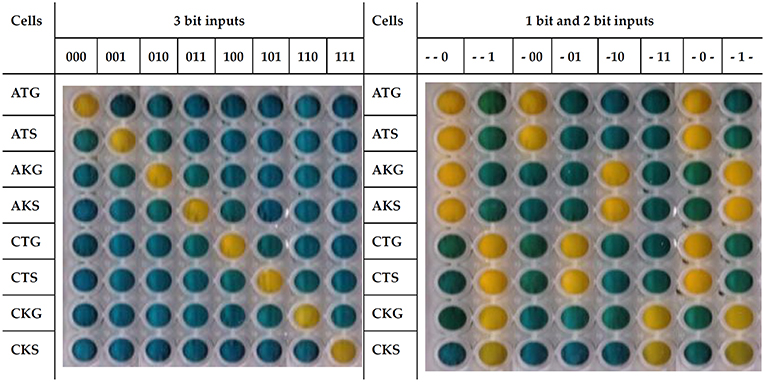
\includegraphics[width=0.7\textwidth]{\dir/figs/fbioe-07-00046-g001.jpg}
  \caption{ParAlleL responding to 1 bit, 2 bit, and 3 bit inputs. ParAlleL subcircuit cells were spatially distributed in different wells (vertically) and exposed to specified 1 bit, 2 bit, or 3 bit inputs (top of each column). Cells were inoculated (1:100) in LB supplemented with 1\% w/v glucose. After 18 h of incubation at 37°C, plates were developed by addition of 0.05 volumes of the developing solution.}
  \label{fig.example}
\end{figure}
In order to further test the ParAlleL system, a digital calculator-like display was designed (Figure 2A). In this case, multiple subcircuit cells are mixed in one well and the global response displays a number from 0 to 7 when the proper binary input is applied. Numbers represent the total eight possible values encoded within 3-bit binary inputs.
\begin{figure}[htbp]
  \centering
  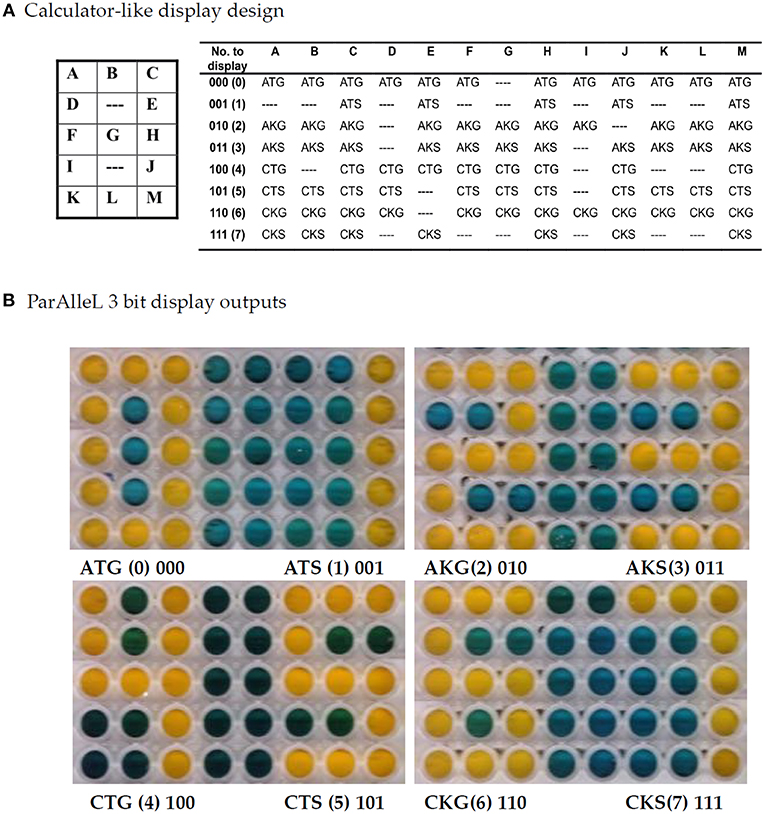
\includegraphics[width=0.7\textwidth]{\dir/figs/fbioe-07-00046-g002.jpg}
  \caption{Digital calculator-like display using 3 bit ParAlleL. Figure shows all numerals from zero to seven based on the 8 binary inputs provided. (A) Subcircuit cells were mixed and distributed in a 3 × 5 matrix and inoculated (1:100) in LB supplemented with 1\%w/v glucose. Plate was developed after 18 h of incubation, by addition of 0.05 volumes of developing solution. (B) Output number results obtained by addition of each 3 bit antibiotic combination.}
  \label{fig.example}
\end{figure}
Input configuration versatility was proven by representing bit A in this case by gentamicin for zero, spectinomycin for one, bit B by kanamycin for zero, tetracycline for one, and bit C by ampicillin for zero, chloramphenicol for one. For instance, once input 110 represented by Ch/Km/Gm is added in the system, the number 6 is displayed (Figure 2).

Finally, a full adder and a full subtractor were designed. A full-adder adds three binary inputs, often denoted as A, B, and Cin, generating a Sum result (S) and a Carry-out (Cout). A full subtractor, on the other hand, has a minuend (X), a subtrahend (Y) and an additional Borrow-in (Bin) as inputs. The subtraction operation produces a difference (D) and a Borrow (Bout) (Figure 3).
\begin{figure}[htbp]
  \centering
  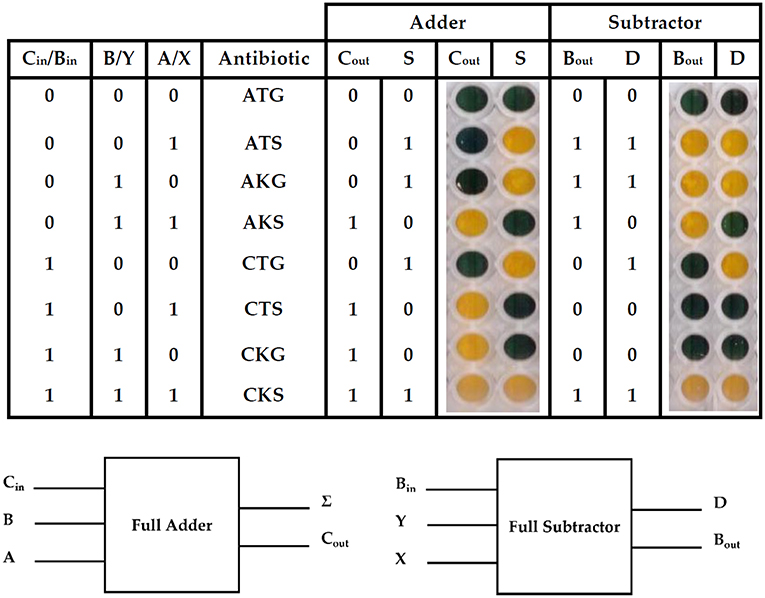
\includegraphics[width=0.7\textwidth]{\dir/figs/fbioe-07-00046-g003.jpg}
  \caption{Full adder and subtractor using the 3 bit ParAlleL system. The figure shows results of addition and subtraction using the ParAlleL for 3 bit system. Cells were mixed as shown in Figure S3 and inoculated (1:100) in LB supplemented with 1\%w/v glucose. After 18 hours of incubation, the plate was developed by addition of the 0.05 volumes of developing solution.}
  \label{fig.example}
\end{figure}
In order to generate the full adder and subtractor, multiple subcircuit cells were mixed and distributed in two different wells (Figure S3). One well represents the solution (S) or difference (D) and a second one the carry (Cout) or borrow (Bout), for the adder and subtractor, respectively (Figure 3). A yellow color represents growth and a positive output 1, a blue color represents no growth and a binary 0 output instead.

\section{\textbf{Conclusions/Discussion}}

Subcircuits that solve complex calculations in parallel have been extensively used for computation in order to reduce the total computation time. Translating this approach to biological systems would allow us to analyze complex processes, currently difficult in synthetic biology, as multiple simple sub-circuits.

In our proof of concept, we present a biological information processing system, ParAlleL, capable of exploiting the parallelism in mixed bacterial cultures. ParAlleL decomposes the analysis of 2 and 3 bit complex inputs, into 4 and 8 sub circuits, respectively (Figure 1). Each sub-circuit corresponds to a different \textit{E. coli} strain carrying a different combination of antibiotic resistance markers (Table S1). As an example, in the 3 bit system the input 000 is represented by the antibiotics ampicillin, tetracycline and gentamicin (Figure 1). When this input is entered into the system, all cells that are not encoded for responding to 000 will die, but cells carrying the proper plasmid combination, pSB4A5, pSB1T3, and pSEVA621 will not (Figures 1.0, 1.1), therefore, a live/dead response (output) is achieved in all sub circuits, the output of each well being one (growth) or zero (failure to grow) (Figure 1.1 and Figure 1.4).

\begin{figure}[htbp]
  \centering
  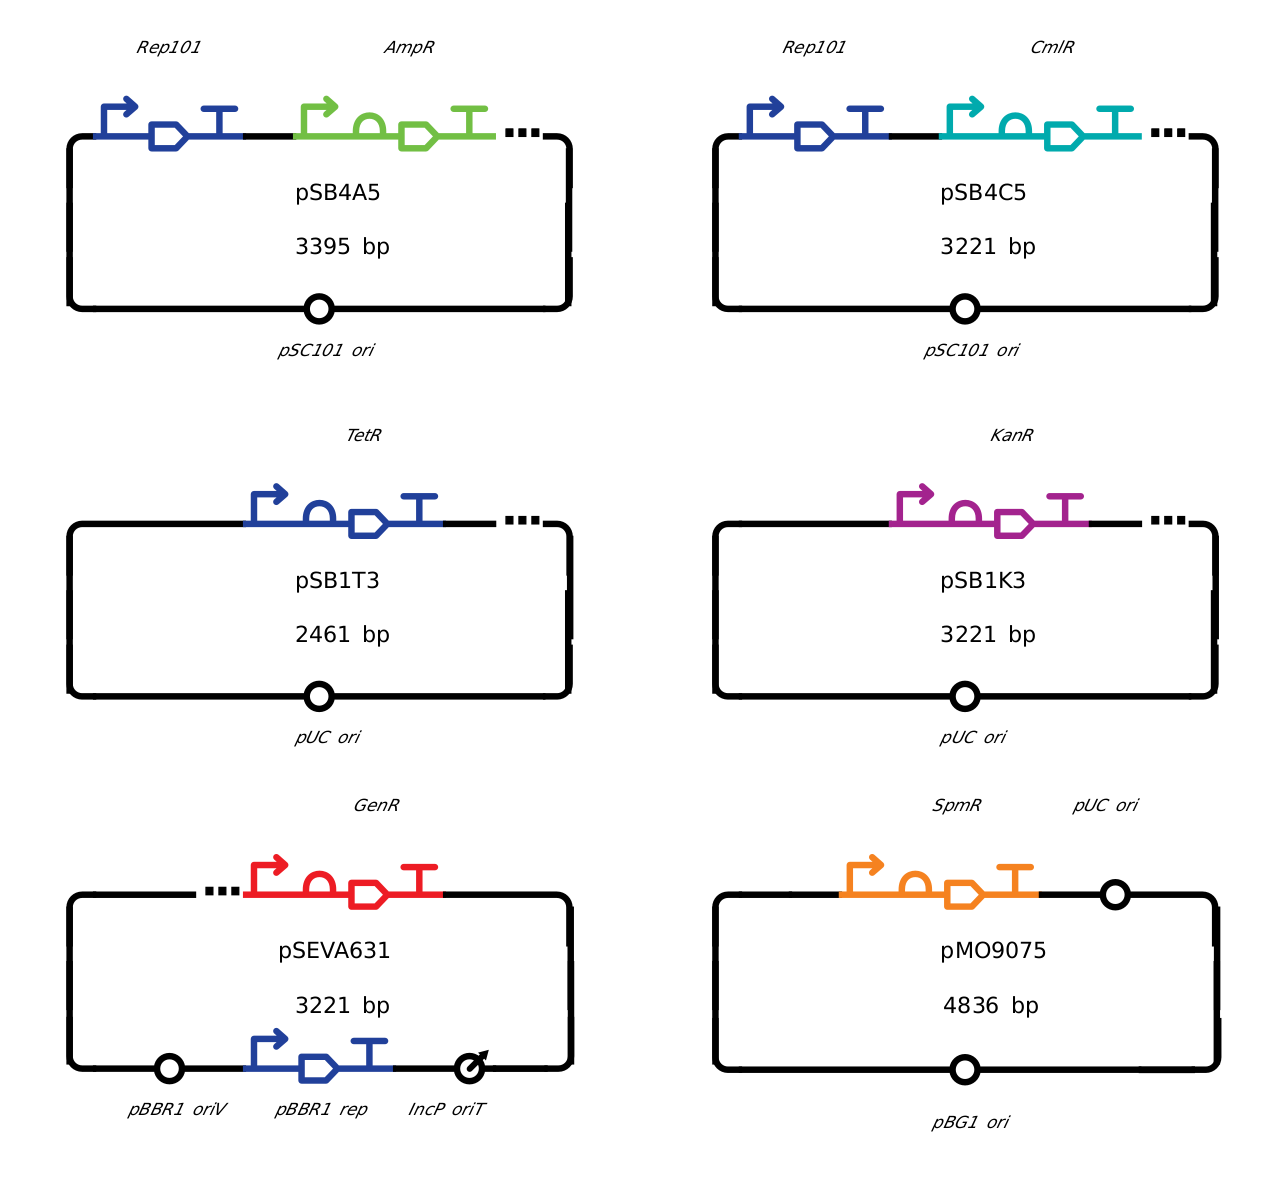
\includegraphics[width=0.7\textwidth]{\dir/figs/plasmids.png}
  \caption{Plasmids carried by subcircuit cells. Plasmids carrying antibiotic resistances for Ampicillin (pSB4A5); Chloramphenicol (pSB4C5); Tetracycline (pSB1T3); Kanamycin (pSB1K3); Gentamicin (pSEVA631) and Spectinomycin (pMO9075) represented in SBOL format. Plasmid sequences available at https://doi.org/10.7488/ds/2497.}
  \label{fig.example}
\end{figure}

ParAlleL uses cellular consortia instead of a single type of cell. A similar approach has been developed by \cite{macia2016implementation,macia2016implementation} using eukaryotic cells, and even showing the possibility of generating transient memory. However, that approach requires a sophisticated design as it relies on a secreted intermediate molecule (hormone-like) that must be kept at the right production level, and that should be previously activated by X (Repressor) and Y (SsrA-tagged protein) degradation. Furthermore, since the output of the circuit is distributed among different consortia, the concentration of the secreted molecule can differ according to the number of cells simultaneously producing it. This kind of multicellular approach and others based on single cells require sophisticated wiring design \cite{silva2008mining,siuti2013synthetic,macia2016implementation,macia2017synthetic}. By contrast, ParAlleL requires very minimal genetic modification and little tuning to obtain reliable outputs (Figures 2, 3).

\begin{figure}[htbp]
  \centering
  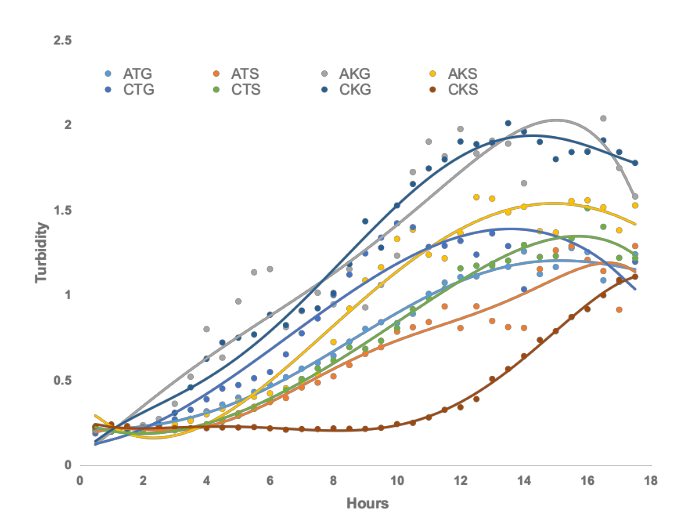
\includegraphics[width=0.7\textwidth]{\dir/figs/growth.png}
  \caption{ParAlleL subcircuit cell growth curves. Growth curves of the 3-bit subcircuit cells in LB + 0.1\% glucose with their respective antibiotic combinations. A: Carbenicilin (100 μg/mL), C: Chloramphenicol (20 μg/mL) T: Tetracycline (10 μg/mL), K: Kanamycin (50 μg/mL), G:
Gentamicin (10 μg/mL). S: Spectinomycin (50 μg/mL). Overnight culture (0.01 volume) was used as inoculum.}
  \label{fig.example}
\end{figure}


The implementation of ParAlleL presented here is simple, but its further development to useful applications presents a number of challenges. Firstly, expansion to 4 bits and beyond would require further well-behaved and non-cross-reacting antibiotic resistance markers, and would probably lead to even greater disparities in growth rate than those observed in the three-bit system (Figure S1). This could be addressed, and the flexibility and usefulness of the system increased, by moving away from direct use of antibiotics to a system using tightly controlled inducible promoters, each controlling a lethal “death gene,” such as \textit{ccdB}, with either the presence or absence of the inducer leading to lethality. In this way the system could be made to respond to different combinations of useful inputs, for example in the construction of multiplexed biosensors.

However, to achieve the full potential of ParAlleL, it will be necessary to generate layered systems in which the output from one layer serves as input to another layer. This might be accomplished via quorum sensing, but the implementation would be rather complex and limited. A more attractive option is to transfer the same concept, using a set of agents which each responds to a single combination of inputs, to an alternative system. For example, the concept could be implemented in a cell-free system, in which inputs may be present as small molecules interacting with transcription factors, or as DNA or RNA oligonucleotides. Outputs from the first layer, in the form of DNA or RNA molecules generated by DNA replication (e.g., PCR) or transcription, could then serve as inputs to a second layer. For example, in a PCR-based approach, one of a set of templates would be amplified based on which primer oligonucleotides were added; the output PCR product could then be processed to generate another set of oligonucleotides, or used directly to initiate priming on a second set of templates via formation of three-way junctions. Alternatively, in a transcription-based system, output RNAs from a first layer computation could act as guide RNAs directing binding of CRISPR-based transcription factors to further templates to generate a new set of guide RNAs, eventually leading to production of an output RNA such as a mRNA leading to translation of a visually detectable signal.

Another interesting aspect of ParAlleL is that, since the final output is the result of a population-based calculation, these systems may show a level of “Byzantine fault tolerance,” allowing reliable outcomes even in the face of levels of noise which are unavoidable in biological systems. This would represent a new level of robustness in biological computation systems.

\section{\textbf{Data Availability}}
All datasets generated for this study are included in the manuscript and/or the supplementary files. More Data is available at https://doi.org/10.7488/ds/2497

\section{\textbf{Acknowledgments}}

The authors acknowledge the valuable assistance of Dr. Louise Horsfall for supplying the pMO9075 plasmid and Dr. Aitor De las Heras for supplying the pSEVA631 plasmid. A pre-print version of the manuscript has been published on bioRxiv (Millacura et al., 2018).
\section{\textbf{Supplementary Material}}

The Supplementary Material for this article can be found online at: https://www.frontiersin.org/articles/10.3389/fbioe.2019.00046/full\#supplementary-material

\renewcommand{\dir}{../chapter2/chapter/}
\chapter{TXO: Transcription-Only genetic circuits as a novel cell-free approach for Synthetic Biology}

\section{\textbf{Abstract }}
\justifying
While synthetic biology represents a promising approach to solve real-world problems, 
the use of genetically modified organisms is a cause of legal and environmental concerns. 
Cell-free systems have emerged as a possible solution but much work is needed to optimize their 
functionality and simplify their usage for Synthetic Biology. 
Here we present TXO, transcription-only genetic circuits, independent of translation or post-translation maturation. 
RNA aptamers are used as reaction output allowing the generation of fast, reliable and simple-to-design transcriptional units.
TXO cell-free reactions and their possible applications are a promising new tool for fast and simple bench-to-market genetic 
circuit and biosensor applications.


\section{\textbf{Introduction }}
\justifying
Cells, including microbial, plant and mammalian cells, have been long engineered for responding to a plethora of environmental factors, benefiting from their intrinsic ability to process the entire cycle from the recognition of a specific target, to analysis of the information, and generation of an output signal \cite{1}. 
However, cell-based systems present also unavoidable disadvantages during their usage, including the risk of releasing genetically modified organisms (GMOs) into the environment, accumulation of mutations and genetic instability, uncontrollable side-reactions within the cell, and issues with viability maintenance during long-term storage \cite{2,3,4,5}.

In order to solve these issues, cell-free systems (CFS), also known as transcription-translation (TX-TL) systems, have emerged as a promising alternative. CFS not only inherit most of the benefits from cell-based systems, but also avoid major challenges that they face. Typically CFS are based on non-living cell-extracts or reconstituted systems that by not presenting a living prospect solve problems related to biosafety, cross-reactivity and long-term functionality maintenance. CFS are rather robust to factors that pose cellular stress, including sensitivity to toxic pollutants and to the typical "overload problem" observed when foreign "genetic circuits" are introduced into the cell \cite{6}.

TX-TL systems share with cells a problem hindering their usage in real-time detection. Response time in TX-TL systems may need a long time for transcription, translation and post-translational maturation to occur, in order to finally produce a detectable signal. For instance, Pardee and colleagues \cite{7} developed a cell-free paper toehold-switch sensor for detection of the Zika virus that takes hours for the final visual results to come out \cite{6}. Paper-based cell-free sensors that detected heavy metals and gamma-hydroxybutyrate by expressing sfGFP needed at least one hour for producing a measurable response \cite{8}. Considering the need for in-situ field analysis, an improvement of cell-free systems response time is necessary \cite{9,10}. 

Since CFS are open and easily modifiable systems \cite{11}, time-consuming translation and post-translational modification can be removed, allowing novel approaches with faster signal generation. Alternative output signals independent of translation and post-translational modification can provide the system with a simpler composition, lower resource requirements and, most importantly, a shorter response time. Here, we introduce a transcription-only (TXO) cell-free system using RNA aptamers as output signals rather than translated proteins. 

Fluorescent RNA aptamers are short ribonucleotide sequences that become fluorescent when bound to specific fluorophores. RNA aptamers, such as Spinach \cite{12}, iSpinach \cite{13} and Broccoli \cite{14} have shown excellent properties for generating bright and stable fluorescence. In the past few years, RNA aptamers have been widely applied in live-cell imaging \cite{15} and biosensing \cite{16}. However, these previously reported aptamer-based sensors acted as both sensing elements (binding to target molecules) and signal generator at the same time \cite{17,18}, requiring aptamers specifically designed for each target.

In TXO systems the functions for input detection (sensing), processing (analysis) and output generation (reporting) are decoupled, creating modular systems where aptamers can be used as universal signal generators. To exemplify the versatility of such system, here we used a simple cell-free extract from the microorganism \textit{Cupriavidus metallidurans} CH34, which carries most of the necessary heavy-metal (e.g., Hg$^{+}$, Pb$^{2+}$, Cu$^{2+}$, Zn$^{2+}$, Ni$^{2+}$, among others) responsive transcription factors and the RNA polymerase which they control \cite{19}. Since all necessary transcription factors are provided directly by the cell-free extract only the synthetic transcription unit must be changed to detect these different metal ions. Combining of the easy to design TXO system, with the high sensitivity of the sensing elements and the fast output signal generation provided by RNA aptamers, TXO is a promising tool for accelerating bench-to-market Synthetic Biology, most specifically where in-situ, simple to design and rapid applications are needed.

\section{\textbf{Methodology }}

\subsection*{Reagents and culture conditions}
Fluorophores DFHBI (Tocris \#5609), DFHO (Tocris \#6434), DMABI and 2-HBI (provided by Dr. Jaffrey's laboratory at Cornell University) were dissolved in DMSO (Fisher Scientific \#BP231) to prepare 2 mM stock solutions (for further information see Table S1).
Our optimised transcription/detection buffer (OTDB) was prepared as a 10X stock as follows: Tris base 400 mM pH 7.5 adjusted with HCl (Sigma-Aldrich, \#T1503); MgCl$_2$\textperiodcentered6(H$_2$O) 60 mM (Sigma-Aldrich, \#M2670); DTT 100 mM (Melford, \#MB1015) and Spermidine 20 mM (Alfa Aesar, \#A19096.03). 
Metal-ion solutions were prepared from soluble salts of analytical grade: CuSO$_4$\textperiodcentered5H$_2$O (Sigma-Aldrich \#C8027), Arsenite NaAsO$_2$ (Sigma-Aldrich \#202673), Pb(NO$_3$)$_2$ (Sigma-Aldrich \#228621), HgCl$_2$ (Sigma-Aldrich \#215465), ZnCl$_2$ (Sigma Aldrich \#229997) and NiCl$_2$\textperiodcentered6H$_2$O (Fisher Scientific \#AC27051) in double-deionised water and filter-sterilised before use. 


\subsection*{Strains and cell-free extract preparation}

\textit{C. metallidurans} CH34 cells were cultivated on a Tris-buffered mineral medium (MM284) \cite{20} supplemented with succinate 0.4 \%w/v, at 30$^{\circ}$C with constant shaking at 180 RPM. \textit{Escherichia coli} JM109 cells were grown on Luria Broth (LB) at 37$^{\circ}$C. 
For cell-extract preparation, cells were collected at middle exponential phase (OD 0.6-0.8) by centrifugation at 3,900 $\times$ \textit{g} and 4$^{\circ}$C for 10 min. Cells were resuspended in one tenth of the centrifuged volume in a non-ionic lysis buffer, which contains Triton X-100 0.1\%v/v (Sigma-Aldrich \#T9284), Tris base (40 mM) adjusted to pH 7.5 with HCl and lysozyme 50 mg/mL (Sigma-Aldrich \#L6876) for 30 min at 4$^{\circ}$C.
The lysed extract was centrifuged at 12,000 $\times$ \textit{g}, 4$^{\circ}$C for 20 min and the supernatant was immediately used or saved at -80$^{\circ}$C for later use.

\subsection*{Construction of RNA aptamers}

Aptamer sequences (see Table \ref{table:01}) protected within the F30 scaffold (upper and lower sections) were synthesised as 120 bp oligonucleotide sequences (Sigma-Aldrich), and then extended using the 5 bp shared on the 3' of each oligonucleotide for the annealing (see Figure \ref{NAR-fig1} and Table S2)
A PCR reaction adding a T7 promoter/terminator pair on each aptamer (see Table \ref{table:01}) was carried out using Q5 High-Fidelity DNA Polymerase (New England Biolabs Inc.(NEB) \#M0491) and the following protocol: 95$^{\circ}$C for 5 min (1 cycle), 95$^{\circ}$C for 20 s, 54$^{\circ}$C for 10s and 72$^{\circ}$C for 20 s (35 cycles), with a final elongation at 72$^{\circ}$C for 5 min. Amplification was analysed in a 1.5 \% (w/v) agarose gel and purified from the PCR reaction using the QIAquick PCR Purification Kit (Qiagen, \#28104), and subsequently cloned in to the pMini-T plasmid using the PCR Cloning Kit (NEB \#E1202). 
Plasmids were extracted from \textit{E.coli} JM109 transformed cells using the QIAprep Spin Miniprep Kit (Qiagen) and sequence verified by Sanger sequencing using the BigDye Terminator v3.1 Cycle Sequencing Kit (Thermo Fisher Scientific) and an Applied Biosystems 3730XL DNA Analyzer (Edinburgh Genomics).

\begin{figure*}[h]
\begin{center}
\hspace*{0cm}
\includegraphics[height=220px]{Figure-1ab.png}
\end{center}
\caption{Schematic diagrams of TXO cell free system with minimal requirements. \textbf{(a)} Sequence and production process of diverse RNA aptamers via PCR, showing addition of BsmBI sites for further Golden Gate manipulation. \textbf{(b)} In a TXO system there are minimal requirements such as an inducer, moderator/repressor, RNA polymerase and a final RNA output herewith represented as a fluorescent aptamer.}
\label{NAR-fig1}
\end{figure*}

\subsection*{Biosensor transcriptional unit design}
Diverse inducible promoters and a T7 terminator were added at the ends of the aptamer F30::iSpinach via PCR \cite{13}. The PCR was carried out using Phusion High-Fidelity DNA Polymerase (NEB \#M0530) and oligonucleotides containing the promoters from clusters \textit{copAB}, \textit{arsBCD} from \textit{E. coli} MG1655 and \textit{merTPAD}, \textit{pbrAB}, \textit{czcN}, \textit{cnrH} from \textit{C. metallidurans} CH34 (see Table S2). Amplified products were analysed and cloned for replication as described above.

\subsection*{RNA aptamer expression and detection.}

Some previous protocols for \textit{in vitro} transcription of fluorescent RNA aptamers \cite{12, 13} include purification and concentration steps that complicate the use of aptamers for real-time detection. A combination of both main steps, expression and detection, was achieved at room temperature (25$^{\circ}$C) by using the OTDB buffer.
\textit{In vitro} transcription and detection assays were carried out using OTDB 1X, NTPs (2 mM each), Fluorophores 10 $\mu$M (see Table \ref{table:01}), NEB T7 RNA Polymerase (1.5 U/$\mu$L), linear target DNA (650 nM), using 15 $\mu$L total reaction volume in 384 Well Small Volume$^{TM}$ LoBase Black Microplates (Greiner Bio-One). 
 Fluorescence was measured using a FluoStar Omega (BMG Labtech) plate reader, 10 mm bandpass, using 20 flashes per well and an orbital averaging of 4 mm, with 5 seconds of orbital shaking prior to each measurement, and filters as close as possible to the wavelength specified in literature (see Table \ref{table:01}). Fluorescence was thereafter imaged using a Safe Imager$^{TM}$ Blue-Light Transilluminator (Invitrogen) with an amber filter unit and a digital camera (Sony, DSC-RX100). 

\subsection*{Heavy metal detection by TXO assays}

Transcriptional regulators MerR (Q5NUU7), PbrR (Q58AJ5), CzcS (Q44007)/CzcR (Q44006), CnrH (P37978), ArsR (Q1LCN6) and CueR (A0A2L0XBJ2) were provided into the working reaction directly in the form of cell extract from \textit{C. metallidurans} CH34 cells (30 \%v/v). 
Reactions were supplemented with increasing concentrations (0.3 $\mu$M, 2 $\mu$M and 7 $\mu$M) of Hg$^{2+}$, Cu$^{2+}$, Co$^{2+}$, Ni$^{2+}$, Pb$^{2+}$ and As$^{3+}$. 
Cell-free metal contact induction was performed in 384 Well Small Volume$^{TM}$ LoBase Black Microplates (Greiner Bio-One) at 25$^{\circ}$C, using DFHBI (10 $\mu$M) as fluorophore, and analysed in a FluoStar Omega (BMG Labtech) plate reader as described above.


\section{\textbf{Results}}
\section*{Results}
\subsection*{Fluorogenic RNA aptamers and TXO systems}

Commonly, cell-free systems are associated with the use of TX-TL systems instead of living cells for the production of valuable compounds or the generation of translational biosensors. Their dependence on translation, however, increases the complexity and cost of the minimal reaction mixture needed for them to work. In order to generate an alternative approach, we evaluated the use of multiple fluorescent RNA aptamers as possible output signals for the generation of transcription-only cell-free systems.

\begin{table}[h]
\tableparts{%
\caption{RNA Aptamers and their respective characteristics
\\}
\label{table:01}%
}{%
\hspace{1.5cm}
\begin{tabular*}{\columnwidth}{@{}llllll@{}}
\toprule
\textbf{Aptamer} & \textbf{Emitted} & \textbf{Size} & \textbf{Ex/Em} & \textbf{Fluorophore} & \textbf{Reference}
\\
& \textbf{Colour} & \textbf{(bp)} & \textbf{(nm)} & & 
\\
\\
\colrule
Broccoli & Green & 47 & 470/530 & DFHBI & \cite{14}
\\
Broccoli2X & Green & 157 & 470/530 & DFHBI & \cite{21}
\\
Spinach2 & Green & 95 & 480/520 & DFHBI & \cite{12}
\\
iSpinach* & Green & 78 & 480/520 & DFHBI & \cite{13}
\\
Corn & Orange & 45 & 480/520 & DFHO & \cite{22}
\\
2-4** & Cyan & 100 & 400/460 & DMABI & \cite{12}
\\
17-3*** & Yellow & 101 & 400/550 & DMABI & \cite{12}
\\
6-8**** & Red & 101 & 400/600 & 2-HBI & \cite{12}
\\
\botrule
\end{tabular*}
}
{\\
\\Ex/Em extracted from respective Ref. 
Hereafter named *Green, **Cyan, ***Yellow, ****Red due to their protection within the F30 scaffold. Further  fluorophores information   available in Table S1}
\end{table}

Eight previously characterised fluorescent aptamers were initially screened (see Table \ref{table:01}). These were synthesised as 120 bp oligonucleotides and amplified in an overlapping PCR using the 5 bp that they share at their 3' end (see Material and Methods, Figure \ref{NAR-fig1} and Table S2). Additionally, unprotected aptamers (Green, Cyan, Yellow, Red, Corn) were inserted within the F30 RNA scaffold, an engineered version of the naturally occurring phi-29 viral RNA three-way junction motif, not cleaved by cellular nucleases \cite{21}. Additionally, BsmBI sites were added at both ends of each aptamer to allow insertion or replacement of the RNA aptamers via Golden Gate assembly if required in future applications (see Figure \ref{NAR-fig1}). RNA expression and fluorescence detection were performed at room temperature (25$^{\circ}$C) in order to simulate field conditions as closely as possible. Furthermore, in order to simplify their use we combined the expression and detection steps by using the novel OTDB buffer (see Materials and Methods), avoiding purification steps needed in some previous cell-free publications. Aptamers were selected primarily by difference in the colour emitted (green, red, orange, yellow, cyan), stability once protected within the F30 scaffold \cite{21}, length, fluorophore needed, and expression level under our previously mentioned experimental conditions (see Table \ref{table:01}). 

The linear PCR-generated fragments can be immediately used for \textit{in vitro} transcription and fluorescence detection. We tested the expression of nine different aptamers with five different fluorophores using a plate reader and an inexpensive blue light/red filter system (see Figure \ref{NAR-fig2}). While previous studies regarded aptamers to be specific for a fluorophore (see Table 1), we have found that cross-reactivity is much higher. As shown in Figure \ref{NAR-fig2}a, Spinach, Broccoli and their derivatives, engineered to bind DFHBI, were found to fluoresce with DMABI and DFHO with their respective colours. Broccoli2X was the most unspecific even increasing the fluorescence of ROX, which we were using as positive fluorescence control. On the other hand, DFHO was the most promiscuous fluorophore, which also displayed background fluorescence with the negative control. 
The aptamer fluorescence appeared very quickly after induction of transcription; after just a few minutes of incubation at room temperature, there was a significant difference between some aptamers and the negative control (see Figure \ref{NAR-fig2}b). However, the fluorescent signal kept increasing for 100 minutes (Figure \ref{NAR-fig2}b), indicating that the RNA polymerase remained active and the NTP pool was not exhausted for this period. Additionally, all F30::aptamers presented high stability over time when left on the bench at room temperature and without further protection. Aptamer-fluorophore complexes were stable for weeks without bleaching or loss of fluorescence (See Figure S1).

\begin{figure*}[ht]
\begin{center}
\includegraphics[height=140px, width=150px]{Figure-2a.png}
\includegraphics[height=140px, width=220px]{Figure-2b.png}
\end{center}
\caption{Fluorescent RNA aptamers expression. \textbf{(a)} Aptamers showing different colours under a blue light/red filter system after plate reader fluorescent measurement (16.5 h) and being observed by naked eye without the need for further equipment. A longer exposed image can be found in Supplementary Figure S1.
\textbf{(b)} Expression of diverse RNA aptamers over time detected at 480/520 nm. Coloured shades represent the variability (MAD) of three independent tests. }
\label{NAR-fig2}
\end{figure*}

\subsection*{TXO cell-free biosensors}
Short aptamers such as the Green aptamer allow incorporation into transcriptional units with ease and simplicity (see Materials and Methods). Considering the stability and optimization of the Green aptamer (F30::iSpinach) for expression under \textit{in vitro} conditions, further experiments were performed with this aptamer. The Green aptamer (F30::iSpinach) was amplified via PCR under the control of diverse heavy metal inducible promoters and the T7 polymersase promoter as control (P\textit{t7}, P\textit{cue}, P\textit{ars}, P\textit{mer}, P\textit{pbr}, P\textit{czc}, P\textit{cnr}, see Material and Methods). Linear PCR products were used in reactions with different heavy metal concentrations (5 $\mu$M, 25 $\mu$M and 100 $\mu$M) with transcription factors and native RNA polymerase supplied from cell lysates (see Figure \ref{NAR-fig3}). Using our TXO cell free system concentrations as low as 2 $\mu$M were detected for lead, mercury, zinc, and arsenite. Nickel, on the other hand, was detected at 0.3 $\mu$M.  All of them reached a 2 fold-change in fluorescence after just 20 min of initiation of the transcription reaction (see Figure \ref{NAR-fig3}) which kept increasing over time reaching after three hours values up to 10-times higher (see Figure S2).

\begin{figure*}[t]
\begin{center}
\hspace*{0cm}
\includegraphics[width=380px]{Figure-3.png}
\end{center}
\caption{Heavy metal detection by TXO Cell-free biosensors. Detection of Pb$^{2+}$, Hg$^{2+}$, Zn$^{2+}$, Ni$^{2+}$, Cu$^{2+}$ and As$^{3+}$
using the TXO reaction Cell-free system and the Green RNA aptamer cloned with each specified promoter (P\textit{pbr}, P\textit{mer}, P\textit{cnr}, P\textit{czc}, P\textit{cop}, and P\textit{ars}). Constructs were induced using increasing concentrations of the specified heavy-metal. Excitation/Emission of 480/520 nm. Data points at 20 minutes; the time course can be found in Supplementary Figure S2. Error bars represent the variability (MAD) of three independent tests.}
\label{NAR-fig3}
\end{figure*}


\section{\textbf{Discussion / Conclusions}}
TXO systems maintain the advantages of cell-free TX-TL systems in terms of uniformity and avoidance of regulatory issues related to live GMOs, and further increase the simplicity and speed of response at the expense of reduced flexibility, since new proteins can not be generated within the system. Hence they are well suited to applications where simplicity and rapid response are paramount; for example, biosensors and diagnostics for use in field and point-of-care applications.
Lack of translational capability means that reporters for system output must be in the form of nucleic acids. We tested eight previously described fluorescent aptamer-fluorophore systems and found that all could generate visible fluorescent responses in an optimized buffer system as a result of transcription with no further processing. Several of the aptamers showed the ability to bind a wider range of fluorophores than what has previously been reported; for example, Broccoli2X binds 4 out of the 5 fluorophores analysed (Figure 2a and S1), surprisingly including ROX (5-Carboxy-X-rhodamine N-succinimidyl ester) commonly used for basal line generation during routine fluorescent assays, such as qPCR. Using TXO systems fluorescent responses can be generated in a matter of minutes, as compared to an hour or more for reported TX-TL systems based on generation of fluorescent proteins or enzymes with chromogenic substrates \cite{6, 23, 24, 25, 26, 27}. Thus we conclude that aptamer-fluorophore complexes are a suitable output for TXO synthetic biology systems. 

A further advantage of TXO systems is simplicity, meaning that they can be very rapidly generated and tested, even more so than TX-TL systems \cite{7}. The aptamer-based reporter genes are small enough that they can be easily generated by annealing and extension of oligonucleotides (see Figure \ref{NAR-fig1}). PCR was used to add metal-responsive promoters to DNA encoding the F30::iSpinach reporter (‘Green’), and the PCR products were used directly for assays, with the necessary transcription factors being supplied by an unpurified lysate from \textit{C. metallidurans} CH34. Fluorescent response to metals was observed within minutes, with detection limits in these unoptimized systems below 0.3 $\mu$M (18 ppb) for nickel, and below 2 $\mu$M for copper (127 ppb), zinc (131 ppb), arsenic(III) (150 ppb), mercury (403 ppb) and lead (414 ppb). No response was observed for arsenic(V), presumably because the system lacked the reducing power necessary to reduce it to arsenic(III), the form actually detected by the ArsR repressor (Data not shown). Further optimization should reduce these limits of detection. Previous works with RNA aptamers for metal sensing, DasGupta et al. mentioned the use of a truncated form of the Spinach aptamer as a Pb$^{2+}$ sensor, but this could have lead to false results at concentrations \textless 2 ppm due to a lack of sensitivity and a weak output response \cite{30}. 

Since TXO systems are considerably simpler than TX-TL systems, with no requirement for ribosomes, tRNA, or associated enzymes, we expect that it will be possible to freeze-dry such systems for storage and distribution as previously reported for TX-TL systems \cite{8, 28}. Fluorescent signals may be further strengthened using alternative fluorophores such as DHFBI-1T \cite{29}. The visibly different colours, as well as different excitation and emission wavelengths for different aptamer-fluorophore complexes, raise the possibility of multiplexed assays as well as more complex approaches such as FRET and quenching. While this publication focuses on the use of aptamers as signal output in a TXO ststem, future research could exploit the advantages of translation independent systems introducing other known functions of RNA molecules. Examples include RNA-based molecule detection (e.g. using riboswitch aptamers) and signal processing (e.g. using RNA-RNA hybridisation networks or crRNA/gRNA) \cite{30, 31,32,33,34,35}. Possible improvements to the already existing technology could also imply the use of other RNA aptamers showing different properties, for instance, by improving the structure and conditions of other aptamers published in the original work by Paige \textit{et al}, which emit fluorescence in different wavelength, i.e. red, yellow, cyan (see Table \ref{table:01} and Figure \ref{NAR-fig2}) or by using ribozymes, such as PS2.M, allowing additional possible transcriptional outputs and broadening the possibilities of TXO systems.

Additionally, TXO systems can be made with no need for GMOs, using in vitro DNA manipulation and non-ionic detergent lysis of wild type ACDPI or Biosafety level 1 cells, plus non toxic chemicals and commercially available enzymes/proteins, so procedures could easily be done in high schools or even at home, leading to a democratization of synthetic biology without the worrying risks of people making bioweapons or causing ecological disasters.
Considering that algorithms are simply a sequence of instructions, typically to solve a class of problems or perform a computation, TXO systems offer a step forward in terms of simplicity, ease of implementation, and rapid response, and may be widely useful in synthetic biology for speeding up and simplifying genetic circuit algorithm design and response.


\section{\textbf{Data Availability}}
All datasets generated for this study are included in the manuscript and/or the supplementary files. More Data is available at 

\section{\textbf{Acknowledgments}}

  
The authors acknowledge the valuable assistance of Dr. Samie R Jaffrey on providing diverse RNA aptamers and fluorophores, Dr. Michael Ryckelynck for providing the iSpinach aptamer and Dr. Simon J. Moore for his help in the cell-free system design. Authors also acknowledge the following funding sources: CONICYT/BC-PhD 72170403 (FM), Biotechnology and Biological Sciences Research Council (BBSRC) [grant number BB/J01446X/1] (MV).

\section{\textbf{Supplementary Material}}


\begin{table}[h]

\tableparts{%
\captionsetup{labelformat=empty}
\caption{\textbf{Table S1:} Fluorophores information
\\}

\label{table:S1}%
}{%\hspace*{-5cm}
\begin{tabular*}{\columnwidth}{@{}lll@{}}
\toprule
Abbreviation & Formula & Chemical name 
\\
\colrule
DFHBI & C$_{12}$H$_{10}$F$_{2}$N$_{2}$O$_{2}$ &  3,5-difluoro-4-hydroxybenzylidene imidazolinone
\\
DMABI* & C$_{14}$H$_{17}$N$_{3}$O$_{1}$ & 4-dimethylaminobenzylidene imidazolinone
\\
2-HBI* & C$_{12}$H$_{12}$N$_{2}$O$_{2}$ &  2-hydroxybenzlidene imidazolinone  
\\
DFHO & C$_{12}$H$_{9}$F$_{2}$N$_{3}$O$_{3}$ & 3,5-difluoro-4-hydroxybenzylidene imidazolinone-2-oxime
\\
ROX & C$_{37}$H$_{33}$N$_{3}$O$_{7}$ & 5-Carboxy-X-rhodamine N-succinimidyl ester 
\\

\botrule
\end{tabular*}
}
{
%\hspace*{-5cm}
\\
\textit{*provided by Dr. Sammie R. Jaffrey's laboratory}}
\end{table}

\begin{figure*} [h] 
\begin{center}
\includegraphics[width=350px]{Figure-S1.png}
\end{center}
\captionsetup{labelformat=empty}
\caption{\textbf{Figure S1:} Fluorescent RNA aptamers observed under a blue  light/red  filter  system. Aptamers  showing  different  colours  under  a  blue  light/red  filter  system  after measurement 16.5 h and being observed by naked eye without the need for further equipment. Picture taken with a Sony, DSC-RX100 camera and aperture}
\label{NAR-figS1}%
\end{figure*}

\begin{table}[h]
\tableparts{%
\captionsetup{labelformat=empty}
\caption{\textbf{Table S2:} Oligonucleotides used
\\}
\label{table:S2}%
}{%
\hspace*{-4cm}
\begin{tabular*}{\columnwidth}{@{}lll@{}}
\toprule
\textbf{Oligo} & \textbf{Name} & \textbf{Sequence}
\\
\\
\colrule
F240 & Cyan_{F30::2-4}Fw &  \MakeLowercase{TGTGGGAGACGCAACTGAATGAACCTAGAGTTATGCCAGGCTCTGAGCCTGCTTCGGCAGGTGCTATGATCGCCAGCGGTAT}
\\
& & \MakeLowercase{GCAGTCCGTAACTAGTCGCGTCTCC}
\\
F241 & Cyan_{F30::2-4}Rv &  \MakeLowercase{GTGGGGAGACGCGACTAGTTACGGACTGCATACCGCTGGCGATCATAGCACCTGCCGAAGCAGGCTCAGAGCCTGGCATAA}
\\
& & \MakeLowercase{CTCTAGGTTCATTCAGTTGCGTCTCC}
\\
F242 & 	Red_{F30::6-8}Fw &  \MakeLowercase{TGTGGGagacgcaactgaatgaaaatggcaaaatattcgagaagctggtctgcttcggcaggattctccaaggggtagatc}
\\
& & \MakeLowercase{gtgtattccgtaactagtcgcgtcTCC}
\\
F243 & Red_{F30::6-8}Rv &  \MakeLowercase{GTGGGgagacgcgactagttacggaatacacgatctaccccttggagaatcctgccgaagcagaccagcttctcgaatattt}
\\
& & \MakeLowercase{tgccattttcattcagttgcgtcTCC}
\\
F244 & Yellow_{F30::17-3}Fw &  \MakeLowercase{TGTGGGagacgcaactgaatgaagagcagtagcgagtagttcacaagagctgcttcggcaggatcttgtaggaagtaaatg}
\\
& & \MakeLowercase{tgcaaatccgtaactagtcgcgtctcC}
\\
F245 & Yellow_{F30::17-3}Rv &  \MakeLowercase{GTGGGgagacgcgactagttacggatttgcacatttacttcctacaagatcctgccgaagcagctcttgtgaactactcgcta}
\\
& & \MakeLowercase{ctgctcttcattcagttgcgtctCC}
\\
F296 & Green_{F30::iSpinach}Fw &  \MakeLowercase{gaattcgcggccgcttCTAGAGTAATACGACTCACTATAGGGTTGCCATGTGTATGTGGGAGACGCGACTACGGTGAGGGTC}
\\
&  &  \MakeLowercase{GGGTCCAGTAGCTTCGGCTACTGTTGAGTAGAGTGTGG}
\\
F297 & Green_{F30::iSpinach}Rv & \MakeLowercase{ctgcagcggccgctactagtaCCCCTCAAGACCCGTTTAGAGGCCCCAAGGGGTTATTTGCCATGAATGATCCCGAAGGATC}
\\
&  &  \MakeLowercase{ATCAGAGTATGTGGGGAGACGTACGGAGCCCACA}
\\
F310 & P_{pbr}::Green Fw &  \MakeLowercase{GAATTCGCGGCCGCTTCTAGAGGGCGTCGGATGGGAGATGTCTTGACTCTATAGTAACTAGAGGGTGTTAAATCGGCAACTT}
\\
&  &  \MakeLowercase{GCCATGTGTATGTGGGAGACGCGACTACGGTGAGGGTC}
\\
F311 & P_{mer}::Green Fw & \MakeLowercase{GAATTCGCGGCCGCTTCTAGAGATCGCTTGACTCCGTACATGAGTACGGAAGTAAGGTTACGCTATCCAATTTCAATTCGAAT}
\\
& & \MakeLowercase{TGCCATGTG}
\\
F312 & P_{cop}::Green Fw & \MakeLowercase{GAATTCGCGGCCGCTTCTAGAGAATTTCTTGACCTTCCCCTTGCTGGAAGGTTTAACCTTTATCACATTGCCATGTGTATGTGG}
\\
& & \MakeLowercase{GAGACGCG}
\\
F313 & P_{ars}::Green Fw & \MakeLowercase{GAATTCGCGGCCGCTTCTAGAGGTATATACACATTCGTTAAGTCATATATGTTTTTGACTTATCCGCTTCGAAGAGAGACACT}
\\
 &  & \MakeLowercase{ACCTGCAACTTGCCATGTGTATGTGGGAGACGCGACT}
\\
F330 & Corn_{F30::Corn}Fw & \MakeLowercase{GATCCTTCGGGATCATTCATGGCAAATAACCCCTTGGGGCCTCTAAACGGGTCTTGAGGGGTACTAGTAGCGGCCGCTGCAG}
\\
& & \MakeLowercase{tactata}
\\
F331 & Corn_{F30::Corn}Rv & \MakeLowercase{CTCCTCAGACCTCCTTCCTCGCGCcgtctCCCACATACACATGGCAACCCTATAGTGAGTCGTATTACTCTAGaagcggccgc}
\\
& & \MakeLowercase{gaattc}
\\
F404 & 	P_{czcN}::GreenFw & \MakeLowercase{GAATTCGCGGCCGCTTCTAGAGggagggcgtctctgggtgtgtgctgaaaatggccaagacagtctatgtcccagaagatg}
\\
&  &  \MakeLowercase{actgtcagattgccgagctTTGCCATGTGTATGTGGGAG}
\\
F405 & P_{cnr}::GreenFw & \MakeLowercase{GAATTCGCGGCCGCTTCTAGAGggaggcctgaagccggaacatcgacctgcttacgatcgcgttcttatcgatgcacTTGCC}
\\
& & \MakeLowercase{ATGTGTATGTGGGAGACG}
\\
F408 & PS2M_Fw & \MakeLowercase{gaattcgcggccgcttCTAGAGTAATACGACTCACTATAGGGGTGGGTAGGGCGGGTTGGATAACCCCTTGGGGCCTCTAA}
\\
&  &  \MakeLowercase{ACGGGTCTTGAGGGGtactagtagcggccgctgcagTAT}
\\
F409 & PS2M_Rv & \MakeLowercase{ATActgcagcggccgctactagtaCCCCTCAAGACCCGTTTAGAGGCCCCAAGGGGTTATCCAACCCGCCCTACCCACCCC}
\\
& & \MakeLowercase{TATAGTGAGTCGTATTACTCTAGaagcggccgcgaattc}
\\
F296-F297 & BBK::P$_{T7}$::Green & \MakeLowercase{gaattcgcggccgcttCTAGAGTAATACGACTCACTATAGGGTTGCCATGTGTATGTGGGAGACGCGACTACGGTGAGGG}
\\
& ::T$_{T7}$::BBK& \MakeLowercase{TCGGGTCCAGTAGCTTCGGCTACTGTTGAGTAGAGTGTGGGCTCCGTAGTCGCGTCTCCCCACATACTCTGATGATCCTTCG}
\\
& & \MakeLowercase{GGATCATTCATGGCAAATAACCCCTTGGGGCCTCTAAACGGGTCTTGAGGGGtactagtagcggccgctgcag}
\\
F313-F297 & BBK::P_{ars}::Greeen & \MakeLowercase{GAATTCGCGGCCGCTTCTAGAGGTATATACACATTCGTTAAGTCATATATGTTTTTGACTTATCCGCTTCGAAGAGAGACAC}
\\
&::T$_{T7}$::BBK & \MakeLowercase{TACCTGCAACTTGCCATGTGTATGTGGGAGACGCGACTACGGTGAGGGTCGGGTCCAGTAGCTTCGGCTACTGTTGAGTAG}
\\
& & \MakeLowercase{AGTGTGGGCTCCGTAGTCGCGTCTCCCCACATACTCTGATGATCCTTCGGGATCATTCATGGCAAATAACCCCTTGGGGCCT}
\\
& & \MakeLowercase{CTAAACGGGTCTTGAGGGGtactagtagcggccgctgcag}
\\
F405-F297 & BBK::P$_{cnr}$::Green & \MakeLowercase{GAATTCGCGGCCGCTTCTAGAGggaggcctgaagccggaacatcgacctgcttacgatcgcgttcttatcgatgcacTTGC}
\\
& ::T$_{T7}$::BBK& \MakeLowercase{CATGTGTATGTGGGAGACGCGACTACGGTGAGGGTCGGGTCCAGTAGCTTCGGCTACTGTTGAGTAGAGTGTGGGCTCCG}
\\
& & \MakeLowercase{TAGTCGCGTCTCCCCACATACTCTGATGATCCTTCGGGATCATTCATGGCAAATAACCCCTTGGGGCCTCTAAACGGGTCTT}
\\
& & \MakeLowercase{GAGGGGtactagtagcggccgctgcag}
\\
F312-F297 & BBK::P$_{cop}$::Green & \MakeLowercase{GAATTCGCGGCCGCTTCTAGAGAATTTCTTGACCTTCCCCTTGCTGGAAGGTTTAACCTTTATCACATTGCCATGTGTATGTG}
\\
& ::T$_{T7}$::BBK& \MakeLowercase{GGAGACGCGACTACGGTGAGGGTCGGGTCCAGTAGCTTCGGCTACTGTTGAGTAGAGTGTGGGCTCCGTAGTCGCGTCTCC}
\\
& & \MakeLowercase{CCACATACTCTGATGATCCTTCGGGATCATTCATGGCAAATAACCCCTTGGGGCCTCTAAACGGGTCTTGAGGGGtactagt}
\\
& & \MakeLowercase{agcggccgctgcag}

\botrule
\end{tabular*}
}
\end{table}

\newpage
\makeatletter
\setlength{\@fptop}{0pt}
\makeatother
\begin{table}[ht!]
\tableparts{%
\label{table:S22}%
}{%
\hspace*{-4cm}
\begin{tabular*}{\columnwidth}{@{}lll@{}}
\toprule
\textbf{Oligo} & \textbf{Name} & \textbf{Sequence}
\\
\\
\colrule
F404-F297 & BBK::P$_{czc}$::Green & \MakeLowercase{GAATTCGCGGCCGCTTCTAGAGggagggcgtctctgggtgtgtgctgaaaatggccaagacagtctatgtcccagaagatg}
\\
&::T$_{T7}$::BBK & \MakeLowercase{actgtcagattgccgagctTTGCCATGTGTATGTGGGAGACGCGACTACGGTGAGGGTCGGGTCCAGTAGCTTCGGCTACTG}
\\
& & \MakeLowercase{TTGAGTAGAGTGTGGGCTCCGTAGTCGCGTCTCCCCACATACTCTGATGATCCTTCGGGATCATTCATGGCAAATAACCCCTT}
\\
& & \MakeLowercase{GGGGCCTCTAAACGGGTCTTGAGGGGtactagtagcggccgctgcag}
\\
F311-F297 & BBK::P$_{mer}$::Green & \MakeLowercase{GAATTCGCGGCCGCTTCTAGAGATCGCTTGACTCCGTACATGAGTACGGAAGTAAGGTTACGCTATCCAATTTCAATTCGAA}
\\
& ::T$_{T7}$::BBK& \MakeLowercase{TTGCCATGTGTATGTGGGAGACGCGACTACGGTGAGGGTCGGGTCCAGTAGCTTCGGCTACTGTTGAGTAGAGTGTGGGCTC}
\\
& & \MakeLowercase{CGTAGTCGCGTCTCCCCACATACTCTGATGATCCTTCGGGATCATTCATGGCAAATAACCCCTTGGGGCCTCTAAACGGGTCT}
\\
& & \MakeLowercase{TGAGGGGtactagtagcggccgctgcag}
\\
F310-F297 & BBK::P$_{pbr}$::Green & \MakeLowercase{GAATTCGCGGCCGCTTCTAGAGGGCGTCGGATGGGAGATGTCTTGACTCTATAGTAACTAGAGGGTGTTAAATCGGCAACTT}
\\
& ::T$_{T7}$::BBK & \MakeLowercase{GCCATGTGTATGTGGGAGACGCGACTACGGTGAGGGTCGGGTCCAGTAGCTTCGGCTACTGTTGAGTAGAGTGTGGGCTCCG}
\\
& & \MakeLowercase{TAGTCGCGTCTCCCCACATACTCTGATGATCCTTCGGGATCATTCATGGCAAATAACCCCTTGGGGCCTCTAAACGGGTCTTGA}
\\
& & \MakeLowercase{GGGGtactagtagcggccgctgcag}
\\
\botrule
\end{tabular*}
}
\end{table}

\begin{figure*} [h] 
\begin{center}
\hspace*{-2.5cm}
\includegraphics[width=500px]{FigureS22.pdf}
\end{center}
\captionsetup{labelformat=empty}
\caption{\textbf{Figure S2:} TXO sensors over time with different metals. Coloured shades represent variability of three independent tests.}
\label{NAR-figS2}%
\end{figure*}
\renewcommand{\dir}{../chapter3/chapter/}
\chapter{Cupria, a novel cell-free system for industrial biotechnology}

\section{\textbf{Abstract }}

Cell-free systems (CFS) are an emerging technology where cell extracts are used instead of living genetically-modified cells, thus, not presenting a "living prospect" applicable to current legal regulations.  Here we show a versatile cell-free system based on the master survivalist bacteria \textit{Cupriavidus  metallidurans} CH34, able of not only sensing environmental variables, such as heavy metals, but also synthesize proteins, produce bioplastics and degrade toxic aromatic compounds. This novel cell-free  chassis  could  become  a  standard  for  mass production considering the versatility and robustness showed once compared with standard \textit{E. coli} cell-free systems. 

lala\footnote{testing a footnote}.

\section{\textbf{Introduction }}

While cell based systems have to be a self-replicating chassis as its greater advantage, cell-free expression systems are a powerful tool in applications where cell based expression systems are too variable, slow, difficult to store or prohibitive due to legislation on the release of genetically modified organisms. 

Since interaction with the surrounding environment is direct

As their very nature is to be a defined, precisely controlled system, their lack of a self-replicating functionality, allows them to function in a limited supply of intracellular supplies such as ATP sources, amino acids and nucleotides. In consequence in vitro protein synthesis is limited by two dimensions: the overall maximum protein amount that can be synthesized with the supplied components, and the time during which the cell free expression system stays active before background processes and chemical deterioration have used up supplies or inactivated the system (\cite{carlson2012cell,bernhard2013cell,kwon2015high}.
\section{\textbf{Methodology }}

\subsection*{Strains and Cell free extract preparation}

\textit{E. coli} MG1655 and \textit{C. metallidurans} CH34 strains were grown on Luria Broth (LB) at 37$^{\circ}$C and 30$^{\circ}$C respectively, both under constant shaking at 180 RPM. Cultures were induced with the respective heavy metal at middle exponential phase and cells collected by centrifugation at 10.000 RPM, 4 C for 5 min. Resuspension was performed using Tris-HCl (40 mM) pH 7.5, followed by a nonionic lysis step using Triton X-100 (0.8\%), Tris-HCl (40 mM) pH 7.5 and lysosime 50 mg/mL. Lysed was centrifuged at 10.000 RPM, 4$^{\circ}$C for 10 min and supernatant was saved at -80$^{\circ}$C or immediately used.

\subsection*{DNA constructs generation}
Promoters from clusters \textit{copAB}, \textit{arsBCD} from E. coli MG1655 and \textit{merTPAD}, \textit{pbrAB} from C. metallidurans CH34 were added by PCR at the 5’ of the pTUB[F30::iSpinach] aptamers using the Q5 High-Fidelity DNA Polymerase (NEB). Transcriptional regulators MerR, PbrR, ArsR and CueR were provided in to the working reaction directly from the cell extract.
pBP, pTUB (Moore et al., 2016), pSB1, pSB4 (iGEM collection), pGEM (Promega), pET28, pET31 (Paige et
al., 2011), ptZ57R/T (Autour et al., 2016), pMO (Kuehl et al., 2014), pSEVA (Silva-Rocha et al., 2013)
plasmids were used as backbones. All constructs generated were confirmed by Sanger sequencing(Edinburgh Genomics). Primer sequences are listed in Appendix 2. Plasmids were digested using
appropriate restriction enzymes (NEB) and excised from agarose 1.3 - 2\% gel, and recovered using a
Quiaquick gel extraction kit (Quiagen). Ligation steps were performed using T4 DNA ligase and 30 fmol of
plasmid per 90 fmol of insert (1:3). Ligations were used to transform chemically competent E. coli JM109
cells selected on the appropiate antibiotic, plasmid DNA was prepared
using a QIAprep Spin Miniprep Kit
(Qiagen) and constructs further confirmed by PCR and Sanger sequencing.
Constructs for expressing crRNA (Figure 10) and the F30 scaffold were synthesized (Sigma-Aldrich) and
cloned in to pBP (Figure 7). All RNA aptamers generated by Paige et al., (2011) and Autour (2017), except
Spinach, were cloned by Golden gate assembly in pTUB flanked by an F30 scaffold (Figure 8). Nullomers 2
(5’ GTCCGAGCGTA 3’) and 5 (5’ ATGTTGATGTTGT 3’) (see Table 6) were cloned flanking the
F30::iSPinach construct in the pGEMTeasy by TA cloning (Figure 11 and 12), using Platinum Taq
polymerase High Fidelity (ThermoFisher). Promoters from the copAB and arsBCD operons from E. coli
MG1655 and merTPAD, pbrAB operons from C. metallidurans CH34 were added by PCR on the 5’ end of
the F30::Broccoli (pET28C) and F30::iSpinach (pTUB) aptamers using Q5 High-Fidelity DNA Polymerase
(NEB). Plasmids were transformed into chemically competent E. coli as prepared by the standard TSS
method (Chung et al., 2014).

\subsection*{Expression and detection of Fluorescent RNA aptamers.}

Although there are standard protocols for in vitro transcription of fluorescent RNA aptamers, these include purification and concentration steps that complicate the entire procedure. A combination of both main steps was achieved at room temperature (25$^{\circ}$C) using our Optimized Transcription/Detection buffer (OTDB): Tris-HCl (40 mM) pH 7.5; MgCl2*6(H2O) (6 mM); DTT (1 mM); Spermidine (2 mM); NTPs (2 mM each); DFHBI (20 uM); NEB T7 RNA polymerase (1.5 U/uL); Template DNA (650 nM). 
Fluorescence was measured using a FluoStar Omega (BMG Labtech) plate reader, excitation 480 nm/ emission 520 nm filters (10 mm bandpass), using 20 flashes per well and an orbital averaging of 4 mm, with 5 seconds of orbital shaking prior each measurement. 

\subsection*{Heavy metal quantification by fluorescence detection}
Stock solutions (100 mM) of HgCl 2 (Sigma-Aldrich), CuSO 4 • 5H 2 O (Sigma-Aldrich), ZnSO 4 • 7H 2 O
(Sigma-Aldrich), CdSO 4 (Sigma-Aldrich), Na 2 HAsO 4 • 7H 2 O (Sigma-Aldrich), Pb(NO 3 ) 2 (VWR), NaAsO 2
(HoneyWell) were prepared and used according to their free metal ion concentration (Table 1).
Table 1: Metal stock solution with their free ion concentrations.
Metal solution Concentration ppm Free Ion Concentration ppm
HgCl 2 100 mM 27152 Hg +2 100 mM 20059
CuSO 4 •5H 2 O 100 mM 24969 Cu +2 100 mM 6355
Pb(NO 3 ) 2 100 mM 33120 Pb +2 100 mM 20720
ZnSO 4 •7H 2 O 100 mM 28756 Zn +2 100 mM 6538
CdSO 4 100 mM 20487 Cd +2 100 mM 11241
Na 2 HAsO 4 •7H 2 O 100 mM 31201 As +5 100 mM 7492
NaAsO2 100 mM 12991 As +3 100 mM 7492

\section{\textbf{Results}}

%\begin{figure}[htbp]
 % \centering
%  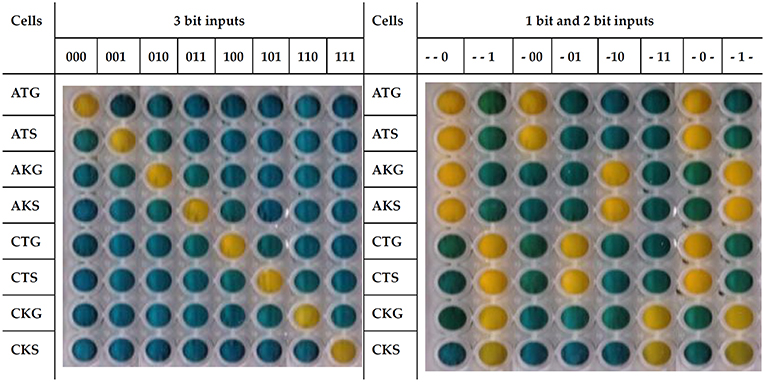
\includegraphics[width=0.7\textwidth]{\dir/figs/fbioe-07-00046-g001.jpg}
%  \caption{ParAlleL responding to 1 bit, 2 bit, and 3 bit inputs. ParAlleL subcircuit cells were spatially distributed in different wells (vertically) and exposed to specified 1 bit, 2 bit, or 3 bit inputs (top of each column). Cells were inoculated (1:100) in LB supplemented with 1\% w/v glucose. After 18 h of incubation at 37$^{\circ}$C, plates were developed by addition of 0.05 volumes of the developing solution.}
 % \label{fig.example}
%\end{figure}

\section{\textbf{Discussion / Conclusions}}
Contamination of the environment with heavy metals is very widespread in many regions. Standard
analytical techniques such as ICP-MS and ICP-OES are highly accurate but require expensive equipment
and highly trained staff. Biosensors offer potential advantages for sensitive, inexpensive field testing, but
those based on live genetically modified cells may be difficult to commercialize for regulatory reasons
(French et al., 2011). Furthermore, as biosensors depend on living organisms, their usability is affected in
real world applications where contamination is widespread and more than one toxic compound is present,
i.e. mining soils that are contaminated with extremely high heavy metal concentrations and multiple aromatic
compounds derived from petrol usage. Cupriavidus metallidurans is an interesting organism for use in this
kind of complex environment (Millacura et al., 2017; Rojas et al 2011), but its use is limited by the same legal
regulations as other biosensors. In this thesis, a cell free extract from this organism will be tested for its
possible use in genetic circuit design, capable of function on complex environments, granting robustness to
the system.
In order to improve the analysis of complex environments, genetic circuits will be generated to
simultaneously analyze the multiple variables present, being the parallel approach a promising design for
decompose the environmental samples into their constituent parts. The modular approach plus the possible
robustness of this system, will allow us to obtain an adaptable system that would not rely on the normal cellprocessing/synthesis machinery (interaction between transcription factors, polymerases, ribosomes, and
other diverse macromolecules), complying with existing and near-future regulations and which can thus be
easily moved into field trials and potentially commercialized.
\section{\textbf{Data Availability}}
All datasets generated for this study are included in the manuscript and/or the supplementary files. More Data is available at https://doi.org/10.7488/ds/2497

\section{\textbf{Acknowledgments}}

Authors acknowledge the following funding sources: CONICYT/BC-PhD 72170403 (FM). 

\section{\textbf{Supplementary Material}}

The Supplementary Material for this article can be found online at: https://www.frontiersin.org/articles/10.3389/fbioe.2019.00046/full\#supplementary-material

\renewcommand{\dir}{../disconclusion/chapter/}
\chapter{Discussion / Conclusions}
Here you finish your thesis as a king/queen and drop the microphone LOL

%========================= Appendix ========================= 
\renewcommand{\chaptermark}[1]{%
 \markboth{\MakeUppercase{%
 \appendixname} \ \thechapter.%
 \ #1}{}}
\renewcommand{\dir}{../appendix/appendix}
\chapter{Appendix}

\begin{center}
\begin{table}[h]
\centering
\caption{Primers designed and synthesised for this thesis} 
\begin{tabular}{ c | c | c }
\hline
  Numb & Name & Sequence \\
 \hline
F208 & Fw-primer-T7-Spi2-BglII & AGATCTTAATACGACTCACTATAGGGGATGTAACTGAATGAAATGGTGAAGGACG	\\
F209 &	Rv-Primer-Spi2-BmtI	& GCTAGCGATGTAACTAGTTACGGAGCTCACACTCT	\\
F210 &	Fw-primerT7-iSpi-BglII &	AGATCTTAATACGACTCACTATAGGGGCGACTACGGTGAGGGTCGGG	\\
F211 &	Rv-Primer-iSpi-BmtI	& GCTAGCGCGACTACGGAGCCCACACTCTAC \\
F212 & 	Fw-F30-2xdBroccoli\-check & GCTCCCACATACTCTGATGATCCAGAC	\\
F213 &	Fw-F30-Broccoli\-check &	CTCCCACATACTCTGATGATCCTTCG	\\
F214 &	Fw-Spinach2\-check &	GATGTAACTGAATGAAATGGTGAAGGA	\\
F215 &	Fw-iSpinach\-check &	ACTACGGTGAGGGTCGGGTCCA	\\
F216 &	GGA-XbaI-T7-prom\-Cpf1\-crRNA-Fw &	CTAGCTATTAATACGACTCACTAT \\	
F217 &	GGA-XbaI-T7-prom\-Cpf1\-crRNA-Rv &	CCCTATAGTGAGTCGTATTAATAG \\	
F218 & GGA-T7-prom-Cpf1\-crRNA\-Fw & CTATTAATACGACTCACTAT	\\
	
F219 &	GGA-T7-prom-Cpf1-crRNA-Rv &	CCCTATAGTGAGTCGTATTA\\	
	
F220 &	GGA-As-crRNA-Fw	 & AGGGTAATTTCTACTCTTGT	\\
	
F221 &	GGA-As-crRNA-Rv	 & ATCTACAAGAGTAGAAATTA\\	
	
F222 &	GGA-Lb-crRNA-Fw &	AGGGTAATTTCTACTAAGTGT	\\
	
F223 &	GGA-Lb-crRNA-Rv &	ATCTACACTTAGTAGAAATTA	\\
	
F224 &	GGA-spacer-Fw &	AGATNNNNNNNNNNNNNNNNNNNN	\\
	
F225 &	GGA-spacer-Rv &	TTATNNNNNNNNNNNNNNNNNNNN	\\
	
F226 &	GGA-T7-terminator-Fw &	ATAACCCCTTGGGGCCTCTAAACGGGTCTTGA \\	
	
F227 &	GGA-T7-terminator-Rv &	CCCCTCAAGACCCGTTTAGAGGCCCCAAGGGG	\\
	
F228 &	GGA-T7-terminator-PstI-Fw &	ATAACCCCTTGGGGCCTCTAAACGGGTCTTGAGGGG	\\
	
F229 &	GGA-T7-terminator-PstI-Rv &	TGCACCCCTCAAGACCCGTTTAGAGGCCCCAAGGGG	\\
	
F230 &	EFX-Lb-Cpf1-Fw &	AGGTCTCAATGAGCAAGCTGGAGAAGTT	\\
	
F231 &	EFX-Lb-Cpf1-Rv &	AGGTCTCAGTGCTTCACGCTGGTCTGGGCGT	\\
	
F232 &	EFX-As-Cpf1-Fw &	AGGTCTCAATGACACAGTTCGAGGGCTT\\	
	
F233 &	EFX-As-Cpf1-Rv &	AGGTCTCAGTTGCGCAGCTCCTGGATGT	\\
	
F234 &	GGA-spacer-Fw &	AGATTGAGACCTTGGTCTCA\\	
	
F235 &	GGA-spacer-Rv &	TTATTGAGACCAAGGTCTCA\\	
	
F236 &	GGA-T7-terminator-PstI-fixed-scar-Fw &	ATA ACC CCT TGG GGC CTC TAA ACG GGT CTT GAG GGG TGC A	\\
	
F237 &	GGA-T7-terminator-PstI-fixed-scar-RV  &	CCC CTC AAG ACC CGT TTA GAG GCC CCA AGG GG	\\
	
F238 &	GGA-XbaI-F30-scaffold-part-PstI-Fw &	CTAGaGGTCTCAAGGGTTGCCATGTGTATGTGGGagacgaacgtctcCCCACATACTCTGATGATCCTTCGGGATCATTCATGGCAAATAAGAGACCTGCA	\\
	
F239 &	GGA-XbaI-F30-scaffold-part-PstI-Rv &	GGTCTCTTATTTGCCATGAATGATCCCGAAGGATCATCAGAGTATGTGGGgagacgttcgtctCCCACATACACATGGCAACCCTTGAGACCT	\\
	
F240 &	Cyan-RNA-2-4-Fw &	TGTGGGAGACGCAACTGAATGAACCTAGAGTTATGCCAGGCTCTGAGCCTGCTTCGGCAGGTGCTATGATCGCCAGCGGTATGCAGTCCGTAACTAGTCGCGTCTCC	\\
	
F241 &	Cyan-RNA-2-4-Rv &	GTGGGGAGACGCGACTAGTTACGGACTGCATACCGCTGGCGATCATAGCACCTGCCGAAGCAGGCTCAGAGCCTGGCATAACTCTAGGTTCATTCAGTTGCGTCTCC	\\
	
F242 &	Red-RNA-6-8-Fw &	TGTGGGagacgcaactgaatgaaaatggcaaaatattcgagaagctggtctgcttcggcaggattctccaaggggtagatcgtgtattccgtaactagtcgcgtctcC	\\
	
F243 &	Red-RNA-6-8-Fw &	GTGGGgagacgcgactagttacggaatacacgatctaccccttggagaatcctgccgaagcagaccagcttctcgaatattttgccattttcattcagttgcgtctCC	\\
	
F244 &	Yellow-RNA-17-3-Fw &	TGTGGGagacgcaactgaatgaagagcagtagcgagtagttcacaagagctgcttcggcaggatcttgtaggaagtaaatgtgcaaatccgtaactagtcgcgtctcC	\\
	
F245 &	Yellow-RNA-17-3-Rv &	GTGGGgagacgcgactagttacggatttgcacatttacttcctacaagatcctgccgaagcagctcttgtgaactactcgctactgctcttcattcagttgcgtctCC	\\
	
F246 &	F30-scaffold-Dw-PstI-Fw &	CCACATACTCTGATGATCCTTCGGGATCATTCATGGCAAATAAGAGACCTGCA	\\
	
F247 &	F30-scaffold-Dw-PstI-Rv &	GGTCTCTTATTTGCCATGAATGATCCCGAAGGATCATCAGAGTAT	\\
	
F248 &	XbaI-F30-scaffold-Up-Fw	& CTAGaGGTCTCAAGGGTTGCCATGTGTA\\	
	
F249 &	XbaI-F30-scaffold-Up-Rv	 & CACATACACATGGCAACCCTTGAGACCt\\	
	
F250 &	Green-RNA-iSpi-Fw &	TGTGGGAGACGCGACTACGGTGAGGGTCGGGTCCAGTAGCTTCGGCTACTGTTGAGTAGAGTGTGGGCTCCGTAGTCGcgtctcc	\\
	
F251 &	Green-RNA-iSpi-Rv &	GTGGGGAGACGCGACTACGGAGCCCACACTCTACTCAACAGTAGCCGAAGCTACTGGACCCGACCCTCACCGTAGTCGCGTCTCC	\\
	
F252 &	gRNA-5'-Biobrick-preffix-Fw	& AGATtggaattcgcggccgcttCTAG\\	
	
F253 &	gRNA-5'-Biobrick-preffix-Rv	& tattCTAGaagcggccgcgaattcca	\\
	
F254 &	gRNA-5'-Biobrick-suffix-Fw &	AGATccggacTGCAGGTCTCTTATTT	\\
	
F255 &	gRNA-5'-Biobrick-suffix-Rv	& TATTAAATAAGAGACCTGCAgtccgg\\	
	
F256 &	T7-As-crRNA-spacer-T7ter-assem-Fw &	CTAGCTATTAATACGACTCACTATAGGGTAATTTCTACTCTTGTAGATTGAGACCTTGGTCTCAATAACCCCTTGGGGCCTCTAAACGGGTCTTGAGGGGTGCA	\\
	
F257 &	T7-As-crRNA-spacer-T7ter-assem-Rv &	CCCCTCAAGACCCGTTTAGAGGCCCCAAGGGGTTATTGAGACCAAGGTCTCAATCTACAAGAGTAGAAATTACCCTATAGTGAGTCGTATTAATAG	\\
	
F258 &	HindIII-SmR-Fw	& ATAAGCTTGAAACGGATGAAGGCACGAACC	\\
	
F259 &	NheI-SmR-Rv &	ATGCTAGCcttttctacgggGTCTGACGCT	\\
	
F260 &	HindIII-ErmM &	ATAAGCTTggccgctactagatgaacgaga	\\
	
F261 &	NheI-ErmM & gcagcggccgctagctagtattac	\\
	
F262 &	Ecoflex seq rev & GCCTTTGAGTGAGCTGATACC	\\
	
F263 &	HindIII-Efx-Fw &	ATAAGCTTgttggcactgatgagggtgtc	\\
	
F264 &	NheI-Efx-Rv	& taGCTAGCGCCTTTGAGTGAGCTGATACC	\\
	
F265 &	HindIII-GmR-Fw &	atAAGCTTCCAGGGGTCCCCAATAATTACGA	\\
	
F266 &	NheI-GmR-Rv	& taGCTAGCGACAACGCGCGGACCGTTGT	\\
	
F267 &	Biobrick-suffix-T7-terminator &	CTGCAGCGGCCGCTACTAGTACCCCTCAAGACCCGTTTAGAGG	\\
	
F268 &	Biobrick-preffix-PbrR &	GAATTCGCGGCCGCTTCTAGAGctagtcgcttggatgggcggt	\\
	
F269 &	Biobrick-preffix-ArsR &	GAATTCGCGGCCGCTTCTAGAGTTAACTGCAAATGTTCTTACTGTCC	\\
	
F270 &	Biobrick-preffix-CueR &	GAATTCGCGGCCGCTTCTAGAGTCACCCTGCCCGATGATGAC	\\
	
F271 &	Biobrick-preffix-MerR &	GAATTCGCGGCCGCTTCTAGAGctaaggcatagccgaacctgc	\\
	
F272 &	MerR-Broccoli2x-Fw &	tcaattcgaaaggacaagcgcTTGCCATGTGTATGTGGGA	\\
	
F273 &	MerR-Broccoli2x-Rv &	TCCCACATACACATGGCAAgcgcttgtcctttcgaattga	\\
	
F274 &	CueR-Broccoli2x-Fw &	TTGCTGGAAGGTTTAACCTTTATCACATTGCCATGTGTATGTGGGAGACG	\\
	
F275 &	CueR-Broccoli2x-Rv &	cGTCTCCCACATACACATGGCAATGTGATAAAGGTTAAACCTTCCAGCAA	\\
	
F276 &	PbrR-Broccoli2x-Fw &	ctagagggtgttaaatcggcaacTTGCCATGtGTATGTGGGAGACG	\\
	
F277 &	PbrR-Broccoli2x-Rv &	cgtCTCCCACATACaCATGGCAAgttgccgatttaacaccctctag	\\
	
F278 &	Pars-Broccoli2x-Fw &	CGAAGAGAGACACTACCTGCAACTTGCCATGtGTATGTGGGAGACG	\\
	
F279 &	Pars-Broccoli2x-Rv &	CGTCTCCCACATACaCATGGCAAGTTGCAGGTAGTGTCTCTCTTCG	\\
	
F280 &	ArsR BS? &	TATGACTTAACGAATGTGTAtaTACACATTCGTTAAGTCATATATGT	\\
	
F281 &	BBK-pre-DE3-Fw	& GAATTCGCGGCCGCTTCTAGAGCAAACTGCGCAACTCGTGAA	\\
F282 &	BamHI-BBK-suf-DE3-Rv &	taGGATCCCTGCAGCGGCCGCTACTAGTAGACAGGCGAATCGCAATCAC	\\
	
F283 &	XbaI-T7-CopB-Rev &	taTCTAGACCCCTCAAGACCCGTTTAGAGGCCCCAAGGGGTTATtcagaaccacatgcgaatacc	\\
	
F284 &	BamHI-T7-CopB-Fw &	atGGATCCATAATACGACTCACTATAGGGtccgactctcttcaaccgacta	\\
	
F285 &	XbaI-T7ter-CopA-Rv &	atTCTAGAATAACCCCTTGGGGCCTCTAAACGGGTCTTGAGGGGtcaggccacaagtacttcgcgga	\\
	
F286 &	BamHI-T7-CopA-Fw &	taGGATCCtaatacgactcactatagggcctgtccggaatgtaatgttcagg	\\
	
F287 &	F287-ArsR-Biotin &	/5Biosg/GTTGCAGGTAGTGTCTCTCTTCG	\\
	
F288 &	ArsR-5'-T7 Fw &	ATTGCGCTCCTGATTGTTGCAGGTAGTGTCTCTCTTCGAAGCGGATAAGTCAAAAACATATATGACTTAATACGACTCACTATAGGG	\\
	
F289 &	ArsR-5'-T7-Rv &	CCCTATAGTGAGTCGTATTAAGTCATATATGTTTTTGACTTATCCGCTTCGAAGAGAGACACTACCTGCAACAATCAGGAGCGCAAT	\\
	
F290 &	ArsR-3'-T7-Fw &	ATTGCGCTCCTGATTGTTGCAGGTAGTGTCTCTCTTCGAAGCGGATAAGTCAAAAACATATATGACTTAACGAATGTGTAAGTAATACGACTCACTATAGGGTTAAGTCATATATGTTTTTGAC	\\
	
F291 &	ArsR-3'-T7-Rv &	GTCAAAAACATATATGACTTAACCCTATAGTGAGTCGTATTACTTACACATTCGTTAAGTCATATATGTTTTTGACTTATCCGCTTCGAAGAGAGACACTACCTGCAACAATCAGGAGCGCAAT	\\
	
F292 &	ArsR-ArsR-Brocc-Fw &	CGTCTCCCACATACaCATGGCAAGTTGCAGGTAGTGTCTCTCTTCGAAGCGGATAAGTCAAAAACATATATGACTTAACGAATGTGTAtaTACACATTCGTTAAGTCATATATGTTTTTG	\\
	
F293 &	ArsR-ArsR-Brocc-Rv &	ATTGCGCTCCTGATTGTTGCAGGTAGTGTCTCTCTTCGAAGCGGATAAGTCAAAAACATATATGACTTAACGAATGTGTAtaTACACATTCGTTAAGTCATATATGTTTTTGACTTATCC	\\
	
F294 &	E. coli rRNA Fw	 & AGT CGT AAC AAG GTA ACC GTA GGG GAA CCT GCG GTT GGA TCA CCT CCT TA	\\
	
F295 &	E coli rRNA Rv	 & TAA GGA GGT GAT CCA ACC GCA GGT TCC CCT ACG GTT ACC TTG TTA CGA CT	\\
	
F296 &	F30-iSpinach Fw &	gaattcgcggccgcttCTAGAGTAATACGACTCACTATAGGGTTGCCATGTGTATGTGGGAGACGCGACTACGGTGAGGGTCGGGTCCAGTAGCTTCGGCTACTGTTGAGTAGAGTGTGG	\\
	
F297 &	F30-iSpinach Rv &	ctgcagcggccgctactagtaCCCCTCAAGACCCGTTTAGAGGCCCCAAGGGGTTATTTGCCATGAATGATCCCGAAGGATCATCAGAGTATGTGGGGAGACGCGACTACGGAGCCCACA	\\
	
F298 &	As-Cpf1-N5-Fw &	ctagaTAATACGACTCACTATAGGGTAATTTCTACTCTTGTAGATATGTTGATGTTGTGGTCTCATAACCCCTTGGGGCCTCTAAACGGGTCTTGAGGGGagagacgctgca	\\
	
F299 &	As-Cpf1-N5-Rv &	gcgtctctCCCCTCAAGACCCGTTTAGAGGCCCCAAGGGGTTATGAGACCACAACATCAACATATCTACAAGAGTAGAAATTACCCTATAGTGAGTCGTATTAT	\\
	
F300 &	As-Cpf1-N2-Fw &	ctagaTAATACGACTCACTATAGGGTAATTTCTACTCTTGTAGATGTCCGAGCGTAGGTCTCATAACCCCTTGGGGCCTCTAAACGGGTCTTGAGGGGagagacgctgca	\\
	
F301 &	As-Cpf1-N2-Rv &	gcgtctctCCCCTCAAGACCCGTTTAGAGGCCCCAAGGGGTTATGAGACCTACGCTCGGACATCTACAAGAGTAGAAATTACCCTATAGTGAGTCGTATTAt	\\
	
F302 &	Cpf1-PAM-N5-Green-Fw &	atagggcaTTTAATGTTGATGTTGTGGTCTCtgagacgttTAATACGACTCACTATAGGG	\\
	
F303 &	Cpf1-PAM-N5-Green-Rv &	atgttccggTTTAATGTTGATGTTGTGGTCTCagagacgcCCCCTCAAGACCCGTTTAGAGG	\\
	 
F304 &	Cpf1-PAM-N2-Green-Fw &	atagggcaTTTAGTCCGAGCGTAGGTCTCtgagacgttTAATACGACTCACTATAGGG	\\
	
F305 &	Cpf1-PAM-N2-Green-Rv &	atgttccggTTTAGTCCGAGCGTAGGTCTCagagacgcCCCCTCAAGACCCGTTTAGAGG\\	
	
F306 &	Cpf1-PAM-N5-mChe-Fw &	acgtctcaGAGACCACAACATCAACATTAAAtgccctattttacagctagc	\\
	
F307 &	Cpf1-PAM-N5-mChe-Rv &	gcgtctctGAGACCACAACATCAACATTAAAccggaacatataaacgcagaaaggccca	\\
	
F308 &	Cpf1-PAM-N2-mChe-Fw &	acgtctcaGAGACCTACGCTCGGACTAAAtgccctattttacagctagc	\\
	
F309 &	Cpf1-PAM-N2-mChe-Rv &	gcgtctctGAGACCTACGCTCGGACTAAAccggaacatataaacgcagaaaggccca	\\
	
F310 &	PbrR-F30::green &	GAATTCGCGGCCGCTTCTAGAGGGCGTCGGATGGGAGATGTCTTGACTCTATAGTAACTAGAGGGTGTTAAATCGGCAACTTGCCATGTGT ATGTGGGAGACGCGACTACGGTGAGGGTC	\\
	
F311 &	merR-F30::green &	GAATTCGCGGCCGCTTCTAGAGATCGCTTGACTCCGTACATGAGTACGGAAGTAAGGTTACGCTATCCAATTTCAATTCGAATTGCCATGTG TATGTGGGAGACGCGACTACGGTGAGGG	\\
	
F312 &	cueR-F30::green &	GAATTCGCGGCCGCTTCTAGAGAATTTCTTGACCTTCCCCTTGCTGGAAGGTTTAACCTTTATCACATTGCCATGTGTATGTGGGAGACGCG ACTACGGTGAGGGTCGGGTCCAGTAGCT	\\
	
F313 &	ArsR-F30::green &	GAATTCGCGGCCGCTTCTAGAGGTATATACACATTCGTTAAGTCATATATGTTTTTGACTTATCCGCTTCGAAGAGAGACACTACCTGCAACT TGCCATGTGTATGTGGGAGACGCGACT	\\
	
F314 &	Primer for Maryia	&

gccgcttCTAGAGTAATACGACTCACTATAGGGTTGCCATGTGTATGTGGGAGACGCGACTACGGTGAGGGTCGGGTCCAGTAGCTTCGGCTACTGTTGAGTAGAGTGTGGGCTCCGTAG\\
	
	
F315 &	Primer for Maryia	&

gccgcttCTAGAGGGAAGTAATTAGGACACACTATAGGTTGCCATGTGTATGTGGGAGACGCGACTACGGTGAGGGTCGGGTCCAGTAGCTTCGGCTACTGTTGAGTAGAGTGTGGGCTC\\
	
	
F316 &	Primer for Maryia	&

gccgcttCTAGAGGGAAGTAATTAGGACACACTATAGGTTAAGTCATATATGTTTTTGACTTGCCATGTGTATGTGGGAGAC\\
	
	
F317 &	Primer for Maryia	 &

gccgcttCTAGAGGGAAGTAATACGACTCACTATAGGGTTAAGTCATATATGTTTTTGACTTGCCATGTGTATGTGGGAGAC\\
	
	
F318 &	Primer for Maryia	&

gccgcttCTAGAGCTCCTGATTGTTGCAGGTAGTGTCTCTCTTCGAAGCGGATAAGTCAAAAACATATATGACTTAATACGACTCACTATAGGGTTGCCATGTGTATGTGGGAGAC\\
	
	
F319 &	Primer for Maryia	 &

gccgcttCTAGAGCTCCTGATTGTTGCAGGTAGTGTCTCTCTTCGAAGCGGATAAGTCAAAAACATATATGACTGGAAGTAATTAGGACACACTATAGGTTGCCATGTGTATGTGGGAGAC\\
	
	
F320 &	Primer for Maryia	 &

gccgcttCTAGAGGGAAGTAATTAGGACACACTATAGGTTGCCATGTGTATGTGGGAGAC\\
	
	
F321 &	Primer for Maryia	 &

gccgcttCTAGAGTAATACGACTCACTATAGGGTTGCCATGTGTATGTGGGAGAC\\
	
	
F322 &	T7::Corn Fw &	GAATTCGCGGCCGCTTCTAGAGTAATACGACTCACTATAGGGTTGCCATGTGTATGTGGGAGACGGCGCGAGGAAGGAGGTCTGAGGAGG TCACTGCGCCGTCTCCCCACATACTCTGAT	\\
	
F323 &	F30::Corn Rv &	TATAGTACTGCAGCGGCCGCTACTAGTACCCCTCAAGACCCGTTTAGAGGCCCCAAGGGGTTATTTGCCATGAATGATCCCGAAGGATCAT CAGAGTATGTGGGGAGACGGCGCAGTGAC	\\
	
F324 &	ArsR::Corn Fw &	GAATTCGCGGCCGCTTCTAGAGGTATATACACATTCGTTAAGTCATATATGTTTTTGACTTATCCGCTTCGAAGAGAGACACTACCTGCAACT TGCCATGTGTATGTGGGAGACGGCGCG	\\
	
F325 &	CueR::Corn Fw &	GAATTCGCGGCCGCTTCTAGAGAATTTCTTGACCTTCCCCTTGCTGGAAGGTTTAACCTTTATCACATTGCCATGTGTATGTGGGAGACGGC GCGAGGAAGGAGGTCTGAGGAGGTCACT	\\
	
F326 &	PbrR::Corn-Fw &	GAATTCGCGGCCGCTTCTAGAGGGCGTCGGATGGGAGATGTCTTGACTCTATAGTAACTAGAGGGTGTTAAATCGGCAACTTGCCATGTGT ATGTGGGAGACGGCGCGAGGAAGGAGGTC	\\
	
F327 & MerR::Corn-Fw &	GAATTCGCGGCCGCTTCTAGAGATCGCTTGACTCCGTACATGAGTACGGAAGTAAGGTTACGCTATCCAATTTCAATTCGAATTGCCATGTG TATGTGGGAGACGGCGCGAGGAAGGAGG	\\
	
F328 & PS2.M Fw & gaattcgcggccgcttCTAGAGTAATACGACTCACTATAGGGTTGCCATGTGTATGTGGGAGACGTGGGTAGGGCGGGTTGGCGTCTCCCCACATACTCTGATGATCCTTCGGGATCATT\\
	
	
F329	& PS2.M Rv & TATATActgcagcggccgctactagtaCCCCTCAAGACCCGTTTAGAGGCCCCAAGGGGTTATTTGCCATGAATGATCCCGAAGGATCATCAGAGTATGTGGGGAGACGCCAACCCGCCC\\
	
	
F330 &	Corn-3-Fw &	GATCCTTCGGGATCATTCATGGCAAATAACCCCTTGGGGCCTCTAAACGGGTCTTGAGGGGTACTAGTAGCGGCCGCTGCAGtactata	\\
	
F331 &	Corn-4-Rv &	CTCCTCAGACCTCCTTCCTCGCGCcgtctCCCACATACACATGGCAACCCTATAGTGAGTCGTATTACTCTAGaagcggccgcgaattc	\\
	
F332 &	RNOC-corn-Fw &	TACTTTGCCATGTGTATGTGGGagacgGCGCGAGGAAGGAGGTCTGAGGAGGTCACTGCGCcgtctcCCCACATACTCTGATGATCCTTCGGGATCATTCATGGCAA\\
F333 &	RNOC-corn-Rv &	AAGCTTGCCATGAATGATCCCGAAGGATCATCAGAGTATGTGGGgagacgGCGCAGTGACCTCCTCAGACCTCCTTCCTCGCGCcgtctCCCACATACACATGGCAA\\
F334 &	RNOC-green-Fw1 &	TACTTTGCCATGTGTATGTGGGAGACGCGACTACGGTGAGGGTCGGGTCCAGTAGCTTCGGCTACTGTTG\\
F335 &	RNOC-green-Fw2 &	AGTAGAGTGTGGGCTCCGTAGTCGCGTCTCCCCACATACTCTGATGATCCTTCGGGATCATTCATGGCAA\\
F336 &	RNOC-green-Rv1 &	AAGCTTGCCATGAATGATCCCGAAGGATCATCAGAGTATGTGGGGAGACGCG\\
F337 &	RNOC-green-Rv2 &	ACTACGGAGCCCACACTCTACTCAACAGTAGCCGAAGCTACTGGACCCGACCCTCACCGTAGTCGCGTCTCCCACATACACATGGCAA\\
F338 &	RNOC-PS2.M-Fw &	TACTTTGCCATGTGTATGTGGGAGACGTGGGTAGGGCGGGTTGGCGTCTCCCCACATACTCTGATGATCCTTCGGGATCATTCATGGCAA\\
F339 &	RNOC-PS2.M-Rv &	AAGCTTGCCATGAATGATCCCGAAGGATCATCAGAGTATGTGGGGAGACGCCAACCCGCCCTACCCACGTCTCCCACATACACATGGCAA\\
F340 &	Prom-CzcN-Fw &	ggagggcgtctctgggtgtgtgctgaaaatggccaagacagtctatgtcccagaagatgactgtcagattgccgagct\\
F341 &	Prom-CzcN-Rv &	agtaagctcggcaatctgacagtcatcttctgggacatagactgtcttggccattttcagcacacacccagagacgcc\\
F342 &	Prom-PbrR-Fw &	ggagggcgtcggatgggagatgtcttgactctatagtaactagagggtgttaaatcggcaac \\
F343 &	Prom-PbrR-Rv &	agtagttgccgatttaacaccctctagttactatagagtcaagacatctcccatccgacgcc \\
F344 &	Prom-CueR-Fw &	ggagAATTTCTTGACCTTCCCCTTGCTGGAAGGTTTAACCTTTATCACA \\
F345 &	Prom-CueR-Rv &	agtaTGTGATAAAGGTTAAACCTTCCAGCAAGGGGAAGGTCAAGAAATT \\
F346 &	Prom-MerR-Fw &	ggagatcgcttgactccgtacatgagtacggaagtaaggttacgctatccaatttcaattcgaa \\
F347 &	Prom-MerR-Rv &	agtattcgaattgaaattggatagcgtaaccttacttccgtactcatgtacggagtcaagcgat \\
F348 &	Prom-ArsR-Fw &	ggagGTAtaTACACATTCGTTAAGTCATATATGTTTTTGACTTATCCGCTTCGAAGAGAGACACTACCTGCAAC \\
F349 &	Prom-ArsR-Rv &	agtaGTTGCAGGTAGTGTCTCTCTTCGAAGCGGATAAGTCAAAAACATATATGACTTAACGAATGTGTAtaTAC \\
F350 &	Prom-CnrH-Fw &	ggaggcctgaagccggaacatcgacctgcttacgatcgcgttcttatcgatgcac \\
F351 &	Prom-CnrH-Rv &	agtagtgcatcgataagaacgcgatcgtaagcaggtcgatgttccggcttcaggc \\
F352 &	Prom-tmoA-Fw &	ggagGTGTTTGGTGTGTTGAGGGCCAGTTGGCCTTAGAAATTATGGA \\
F353 &	Prom-tmoA-Rv &	agtaTCCATAATTTCTAAGGCCAACTGGCCCTCAACACACCAAACAC \\
F354 &	Prom-PhyZ-Fw &	ggagATAGCTCTCCCACCTGAAATCACGAGACAACGCACACGCACCGCGATGTGCGGCG \\
F355 &	Prom-PhyZ-Rv &	agtaCGCCGCACATCGCGGTGCGTGTGCGTTGTCTCGTGATTTCAGGTGGGAGAGCTAT \\
F356 & 	Prom-TomA0-Fw &	ggagAGGCTCATTTCTGCCGATGGGACGCGACTTGCTTTGA \\
F357 &	Prom-TomA0-Rv &	agtaTCAAAGCAAGTCGCGTCCCATCGGCAGAAATGAGCCT \\
F358 &	Prom-tomD-Fw &	ggagGGTTGTTAAGGGAAATCAAGTTATTGCTCGTTGCCGGATACTGGA \\
F359 &	Prom-tomD-Rv &	agtaTCCAGTATCCGGCAACGAGCAATAACTTGATTTCCCTTAACAACC \\
F360 &	Prom-poxR-Fw &	ggagGCAACGCCGGATGCCGTGCTAGGCTACGCAAAAACGAGGCTCGAAAG \\
F361 &	Prom-poxR-Rv &	agtaCTTTCGAGCCTCGTTTTTGCGTAGCCTAGCACGGCATCCGGCGTTGC \\
F362 &	Prom-catA1-Fw &	ggagCAGTCCGCTGTTCCGCTCACTCTGAAGTATTTCCACCACAAA \\
F363 &	Prom-catA1-Rv &	agtaTTTGTGGTGGAAATACTTCAGAGTGAGCGGAACAGCGGACTG \\
F364 &	Prom-catA2-Fw &	ggagcctcgatacgggtttatacccacagagcattaaccgaccgatcattcgacccccaccaaagagacatttcggagtgagac \\
F365 &	Prom-catA2-Rv &	agtagtctcactccgaaatgtctctttggtgggggtcgaatgatcggtcggttaatgctctgtgggtataaacccgtatcgagg \\
F366 &	Prom-tomR-Fw &	ggaggttccctcctcaggaaatcgccagtcagggctctttcttaaaagttcatcgtctcgcacgctctcaccgggtgcgtaaac \\
F367 &	Prom-tomR-Rv &	agtagtttacgcacccggtgagagcgtgcgagacgatgaacttttaagaaagagccctgactggcgatttcctgaggagggaac \\
CF &	fD1	 & ccgaattcgtcgacaacAGAGTTTGATCCTGGCTCAG \\
CF	& rD1 &	cccgggatccaagcttAAGGAGGTGATCCAGCC  \\
F368 &	gRNA LI 3to5 Fw	 & AGCGTTACTCTAGAAAGAGGAGAAAGGATCC \\
F369 &	gRNA LI 3to5 Rv	& GGAGGGATCCTTTCTCCTCTTTCTAGAG \\
F370 &	gRNA LI 5to3 Fw	& GGAGTTACTCTAGAAAGAGGAGAAAGGATCC \\
F371 &	gRNA LI 5to3 Rv	& AGCGGGATCCTTTCTCCTCTTTCTAGAGTAA \\
F372 &	gRNA LI T3 3to5 Fw	& AGTTTCTCGAGCTAGAGACTAGTGGATCC \\
F373 &	gRNA LI T3 3to5 Rv	& CGGGATCCACTAGTCTCTAGCTCGAGAAA \\
F374 &	gRNA LI T3 5to3 Fw & GGTTTCTCGAGCTAGAGACTAGTGGATCC \\
F375 &	gRNA LI T3 5to3  Fw	& AGCGGGATCCACTAGTCTCTAGCTCGAGAAA \\
F376 &	gRNA Strhkendl 3to5 Fw	& CGTTTAGTGATAAGTGGAATGCCATGTGGA \\
F377 &	gRNA Strhkendl 3to5 Rv &	GGAGTCCACATGGCATTCCACTTATCACTAAA \\
F378 &	gRNA Strhkendl 5to3 Fw	& GGAGTTTAGTGATAAGTGGAATGCCATGTGGA \\
F379 &	gRNA Strhkendl 5to3 Fw	& AGCGTCCACATGGCATTCCACTTATCACTAAA \\
F380 &	gRNA Zetsche 3to5 Fw &	AGCGTTTAGAGAAGTCATTTAATAAGGCCACTG \\
F381 &	gRNA Zetsche 3to5 Rv &	TTTAGAGAAGTCATTTAATAAGGCCACTG \\
F382 &	gRNA Zetsche 5to3 Fw &	GGAGTTTAGAGAAGTCATTTAATAAGGCCACTG \\
F383 &	gRNA Zetsche 5to3 Fw &	AGCGCAGTGGCCTTATTAAATGACTTCTCTAAA \\
F384 &	AS crRNA Li1 Fw &	GGAGTAATACGACTCACTATAGGGTAATTTCTACTCTTGTAGATCTCTAGAAAGAGGAGAAAGGATCCATAACCCCTTGGGGCCTCTAAACGGGTCTTGAGGGGTCTA \\
F385 &	AS crRNA Li1 Rv &	AGCGTAGACCCCTCAAGACCCGTTTAGAGGCCCCAAGGGGTTATGGATCCTTTCTCCTCTTTCTAGAGATCTACAAGAGTAGAAATTACCCTATAGTGAGTCGTATTA \\
F386 &	AS crRNA Li3 Fw &	GGAGTAATACGACTCACTATAGGGTAATTTCTACTCTTGTAGATTCGAGCTAGAGACTAGTGGATCCATAACCCCTTGGGGCCTCTAAACGGGTCTTGAGGGGTCT \\
F387 &	AS crRNA Li3 Rv &	AGCGAGACCCCTCAAGACCCGTTTAGAGGCCCCAAGGGGTTATGGATCCACTAGTCTCTAGCTCGAATCTACAAGAGTAGAAATTACCCTATAGTGAGTCGTATTA \\
F388 &	AS crRNA Strhkendl Fw &	GGAGTAATACGACTCACTATAGGGTAATTTCTACTCTTGTAGATAGTGATAAGTGGAATGCCATGTGGAATAACCCCTTGGGGCCTCTAAACGGGTCTTGAGGGG \\
F389 &	AS crRNA Strhkendl Rv &	AGCGCCCCTCAAGACCCGTTTAGAGGCCCCAAGGGGTTATTCCACATGGCATTCCACTTATCACTATCTACAAGAGTAGAAATTACCCTATAGTGAGTCGTATTA \\
F390 &	AS crRNA ZETCHE Fw &	GGAGTAATACGACTCACTATAGGGTAATTTCTACTCTTGTAGATGAGAAGTCATTTAATAAGGCCACTATAACCCCTTGGGGCCTCTAAACGGGTCTTGAGGGG \\
F391 &	AS crRNA ZETCHE Rv &	CCCCTCAAGACCCGTTTAGAGGCCCCAAGGGGTTATAGTGGCCTTATTAAATGACTTCTCATCTACAAGAGTAGAAATTACCCTATAGTGAGTCGTATTA \\
F392 &	LB crRNA Li1 Fw &	GGAGTAATACGACTCACTATAGGGTAATTTCTACTAAGTGTAGATCTCTAGAAAGAGGAGAAAGGATCCATAACCCCTTGGGGCCTCTAAA \\
F393 &	LB crRNA Li1 Rv &	AGCGTTTAGAGGCCCCAAGGGGTTATGGATCCTTTCTCCTCTTTCTAGAGATCTACACTTAGTAGAAATTACCCTATAGTGAGTCGTATTA \\
F394 &	LB crRNA Li3 Fw &	GGAGTAATACGACTCACTATAGGGTAATTTCTACTAAGTGTAGATTCGAGCTAGAGACTAGTGGATCCATAACCCCTTGGGGCCTCTAAA \\
F395 &	LB crRNA Li3 Rv &	AGCGTTTAGAGGCCCCAAGGGGTTATGGATCCACTAGTCTCTAGCTCGAATCTACACTTAGTAGAAATTACCCTATAGTGAGTCGTATTA \\
F396 &	LB crRNA Strhkendl Fw &	GGAGTAATACGACTCACTATAGGGTAATTTCTACTAAGTGTAGATAGTGATAAGTGGAATGCCATGTGGAATAACCCCTTGGGGCCTCTAAA \\
F397 &	LB crRNA Strhkendl Rv &	AGCGTTTAGAGGCCCCAAGGGGTTATTCCACATGGCATTCCACTTATCACTATCTACACTTAGTAGAAATTACCCTATAGTGAGTCGTATTA \\
F398 &	LB crRNA ZETCHE Fw &	GGAGTAATACGACTCACTATAGGGTAATTTCTACTAAGTGTAGATGAGAAGTCATTTAATAAGGCCACTATAACCCCTTGGGGCCTCTAAA \\
F399 &	LB crRNA ZETCHE Rv &	AGCGTTTAGAGGCCCCAAGGGGTTATAGTGGCCTTATTAAATGACTTCTCATCTACACTTAGTAGAAATTACCCTATAGTGAGTCGTATTA \\
J057 &	T7-promoter-fw  &
	taatacgactcactataggg \\
J058 &	T7-promoter-rv	 & gctagttattgctcagcgg \\
J059 &	M13-fw-17 &	GTTTTCCCAGTCACGAC \\
J060 &	M13-rev-17 &	CAGGAAACAGCTATGAC \\
J061 &	M13-fw-24 &	TCACACAGGAAACAGCTATGAC \\
J062 &	M13-rev-24 &	CGCCAGGGTTTTCCCAGTCACGAC \\
MV02 &	Ecoflex seq fw	 & GCCTTTGAGTGAGCTGATACC \\
MV01 &	Ecoflex seq rev	& TATCACGAGGCAGAATTTCAG \\
MV093 &	PS1	 & AGGGCGGCGGATTTGTCC \\
MV094 &	PS2	 & GCGGCAACCGAGCGTTC \\
MV095 &	PS3	 & GAACGCTCGGTTGCCGC \\
MV096 &	PS4	 & CCAGCCTCGCAGAGCAGG \\
MV097 &	PS5	& CCCTGCTTCGGGGTCATT \\
MV098 &	PS5	& GGACAAATCCGCCGCCCT \\
F400 & BBK FW	& Gaattcgcggccgcttctagag \\
F401 &	BBK RV &	ctgcagcggccgctactagta \\
BH5	& Bethan's Primer 5 &	atgaattctgctctagagtaatacgactcactatagggAAggAGGTACTATGGCCACTGATTTTTCAAAG \\
F402 &	PS2M clean Fw &	gaattcgcggccgcttCTAGAGTAATACGACTCACTATAGGGGTGGGTAGGGCGGGTTGGATAACCCCTTGGGGCCTCTAAACGGGTCTTGAGGGGtactagtagcggccgctgcag \\
F403 &	PS2M clean RV &	ctgcagcggccgctactagtaCCCCTCAAGACCCGTTTAGAGGCCCCAAGGGGTTATCCAACCCGCCCTACCCACCCCTATAGTGAGTCGTATTACTCTAGaagcggccgcgaattc \\
F404 &	CzcN-F30::green F340 &	GAATTCGCGGCCGCTTCTAGAGggagggcgtctctgggtgtgtgctgaaaatggccaagacagtctatgtcccagaagatgactgtcagattgccgagctTTGCCATGTGTATGTGGGAG \\
F405 &	CnrH-F30::green F350 &	GAATTCGCGGCCGCTTCTAGAGggaggcctgaagccggaacatcgacctgcttacgatcgcgttcttatcgatgcacTTGCCATGTGTATGTGGGAGACG \\
F406 &	pMini T Fw &	ACCTGCCAACCAAAGCGAGAAC \\ 
F407 &	pMini T Rv &	TCAGGGTTATTGTCTCATGAGCG \\
F408 &	PS2M TU clean Fw &	gaattcgcggccgcttCTAGAGTAATACGACTCACTATAGGGGTGGGTAGGGCGGGTTGGATAACCCCTTGGGGCCTCTAAACGGGTCTTGAGGGGtactagtagcggccgctgcagTAT \\
F409 &	PS2M TU clean Rv &	ATActgcagcggccgctactagtaCCCCTCAAGACCCGTTTAGAGGCCCCAAGGGGTTATCCAACCCGCCCTACCCACCCCTATAGTGAGTCGTATTACTCTAGaagcggccgcgaattc \\

\end{tabular}
\end{table}

	


\begin{table}[h]
\centering
\caption{ParAlleL 3 bit Full adder/subtractor design}
\begin{tabular}{ c c | c c | c c }

\hline
  & & Adder & & Subtractor & \\
 \hline

 Input & Antibiotic & Cout & S & Bo & D \\  
 000 & ATG & --- & --- & --- & ---   \\
  001 & ATS & --- & +++ & +++ & +++ \\
   010 & AKG & --- & +++ & +++ & +++  \\
    011 & AKS & +++ & --- & +++ & ---  \\
     100 & CTG & --- & +++ & --- & +++  \\
      101 & CTS & +++ & --- & --- & ---  \\
       010 & CKG & +++ & --- & --- & ---  \\
        111 & CTG & +++ & +++ & +++ & +++  \\
\end{tabular}
Cells added in specified wells carry resistance markers for:\\
\textbf{ATG:} Ampicilin, Tetracycline, Gentamicin.\\ 
\textbf{ATS:} Ampicilin, Tetracycline, Spectinomycin.\\
\textbf{AKG:} Ampicillin, Kanamycin, Gentamicin.\\
\textbf{AKS:} Ampicillin, Kanamycin, Spectinomycin.\\
\textbf{CTG:} Chloramphenicol, Tetracycline, Gentamicin.\\
\textbf{CTS:} Chloramphenicol, Tetracycline, Spectinomycin.\\
\textbf{CKG:} Chloramphenicol, Kanamycin, Gentamicin.\\
\textbf{CKS:} Chloramphenicol, Kanamycin, Spectinomycin.\\
\end{table}
\begin{table}[h]
\centering
\caption{Plasmids used for generating ParAlleL subcircuit strains.}
\begin{tabular}{ c c c c c }

\hline
  Plasmid & Antibiotic marker & ORI & Copy number & Reference \\
 \hline

 pSB4A5 & AmpR & pSC101 & 5 & http://parts.igem.org/Part:pSB4A5 \\
 pSB4C5 & CmlR & pSC101 & 5 & http://parts.igem.org/Part:pSB4C5  \\
  pSB1T3 & TetR & pMB1(der) & 100-300 & http://parts.igem.org/Part:pSB1T3 \\
   pSB1K3 & KanR & pMB1(der) & 100-300 & http://parts.igem.org/Part:pSB1K3  \\
    pSEVA631 & GenR & pBBR1 & medium & https://www.ncbi.nlm.nih.gov/nucco
re/JX560348  \\
     pMO9075 & SpmR & pBG1 & low & Keller, et al., 2011  \\
      
\end{tabular}

\end{table}

\begin{table}[h]
\centering
\caption{Antibiotics and resistance cassettes used on ParAlleL.}
\begin{tabular}{ c c c c }

\hline
  Antibiotic & Class & Mode of action & Resistance \\
 \hline

Ampicillin & $\beta$-lactam & Bactericidal; Inhibits cell wall synthesis & $\beta$-lactamase (bla) gene  \\
 Kanamycin & Aminoglycoside & Bactericidal; Binds 30S ribosomal subunit; causes mistranslation  & Neomycin phosphotransferase II \\
  Chloramphenicol & Chloramphenicol & Bacteriostatic; Binds 50S  ribosomal subunit; inhibits peptidyl & Chloramphenicol
acetyl transferase translocation \\
   Tetracycline & Tetracycline & Bacteriostatic; Binds 16S ribosomal subunit; inhibits protein synthesis (elongation step)
   & Tetracycline efflux protein   \\
    Gentamicin & Aminoglycoside & Irreversibly binding the 30S subunit of the bacterial ribosome & Gentamicin-3-N-acetyltransferase   \\
     Spectinomycin & Aminocyclitol & It binds to the 30S and interrupts protein synthesis affecting 16S RNA & Spectinomycin adenyltransferase  \\
      
\end{tabular}

\end{table}

\begin{table}[h]
\caption{Plasmid incompatibility groups.}
\centering
\begin{tabular}{ c c c }
\hline
  Incompatibility group & Regulation & Comment \\
 \hline
pBR322/ColE1/pMB1 & Inhibitor-target RNA I & Control processing of pre-RNAII into primer  \\
 IncFII, pT181 & RNA & Affecting synthesis of RepA protein \\
  R6K*, P1, F, pSC101, Rts1, P15A*, RK2 & Iteron binding & Sequestering of RepA protein  \\
      
\end{tabular}

\end{table}
\end{center}






%========================= BIBLIOGRAPHY ========================= 
\ifthenelse{\boolean{edthesis}}
 {
 \begin{singlespace}
}
{
  \backmatter
}
\def\bibname{References}
%\tocotherhead{References}
\addcontentsline{toc}{chapter}{References}
\bibliography{thesis}
\ifthenelse{\boolean{edthesis}}
 {
  \end{singlespace}
 }{}
%========================= Papers ========================= 
\addcontentsline{toc}{chapter}{
Published papers}
\renewcommand{\dir}{../papers/}
\backmatter
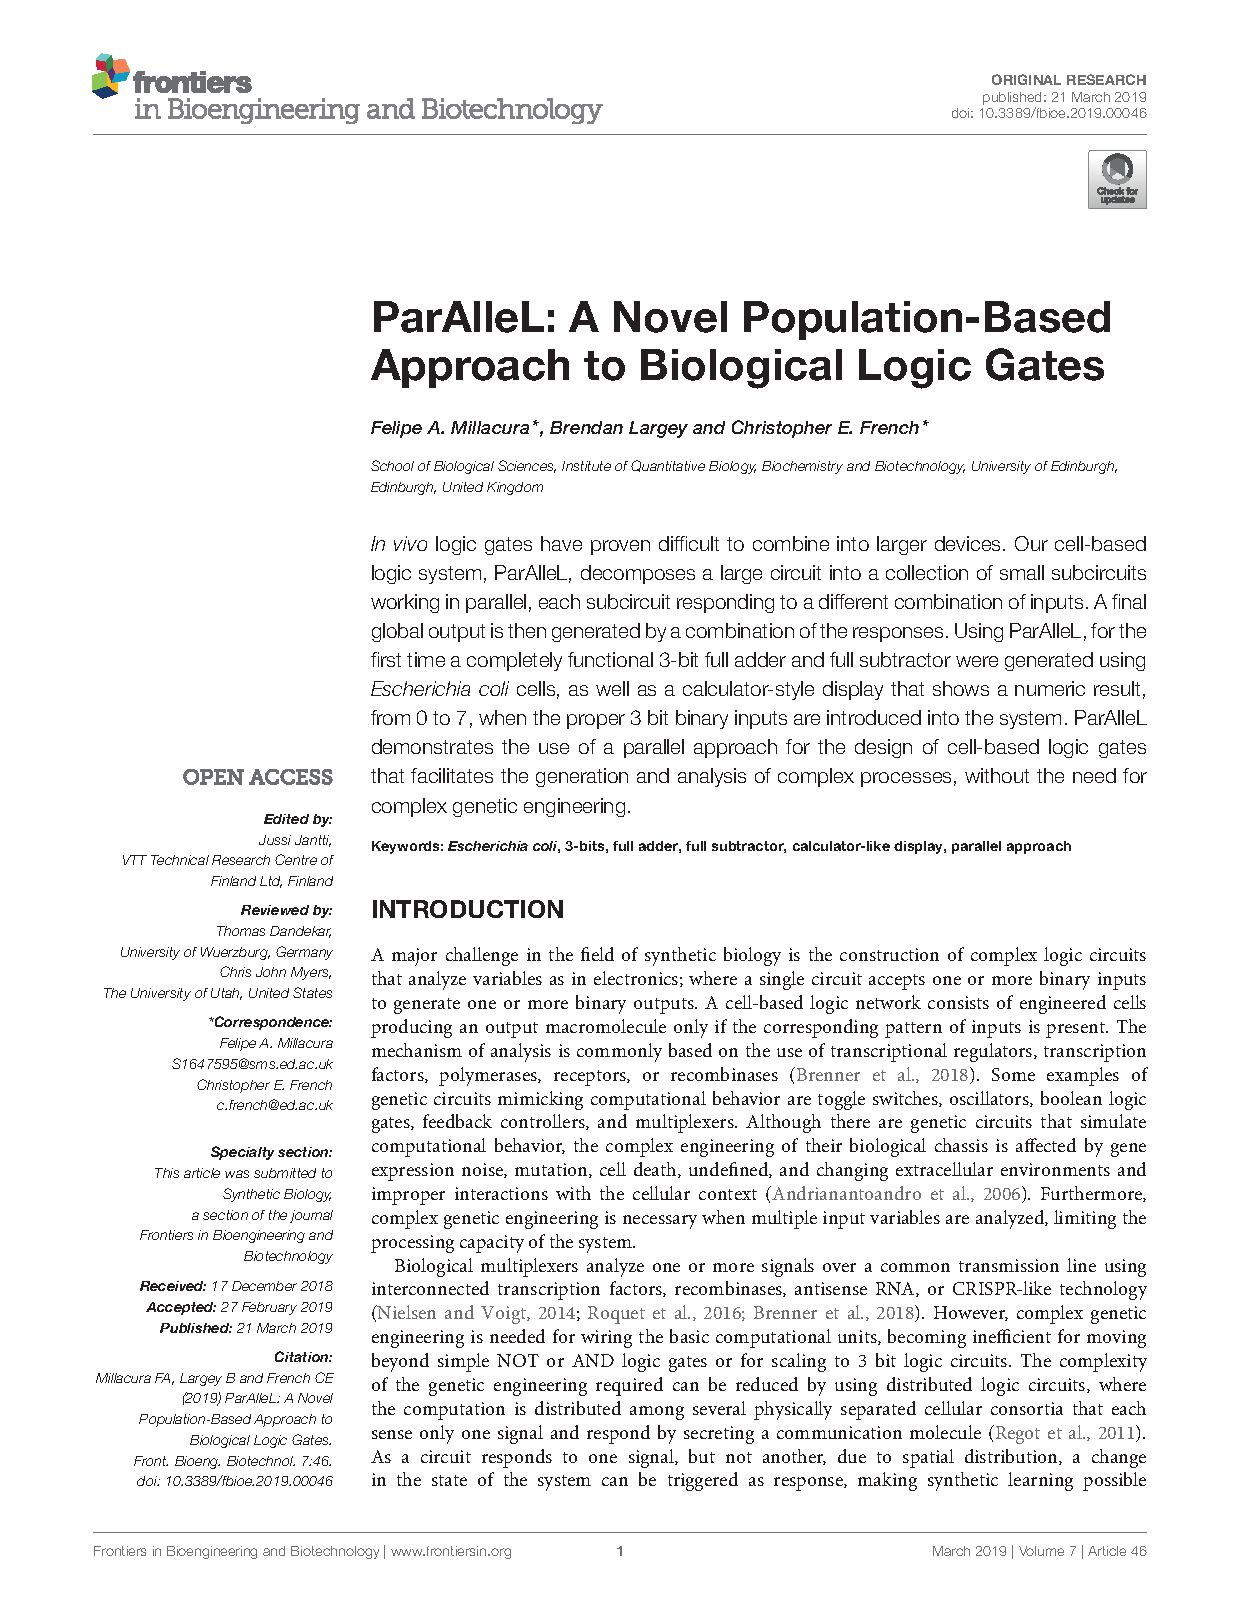
\includepdf[pages=-, width=\paperwidth,height=\paperheight, offset= 20 -20]
{\dir/fbioe-07-00046(1).pdf}
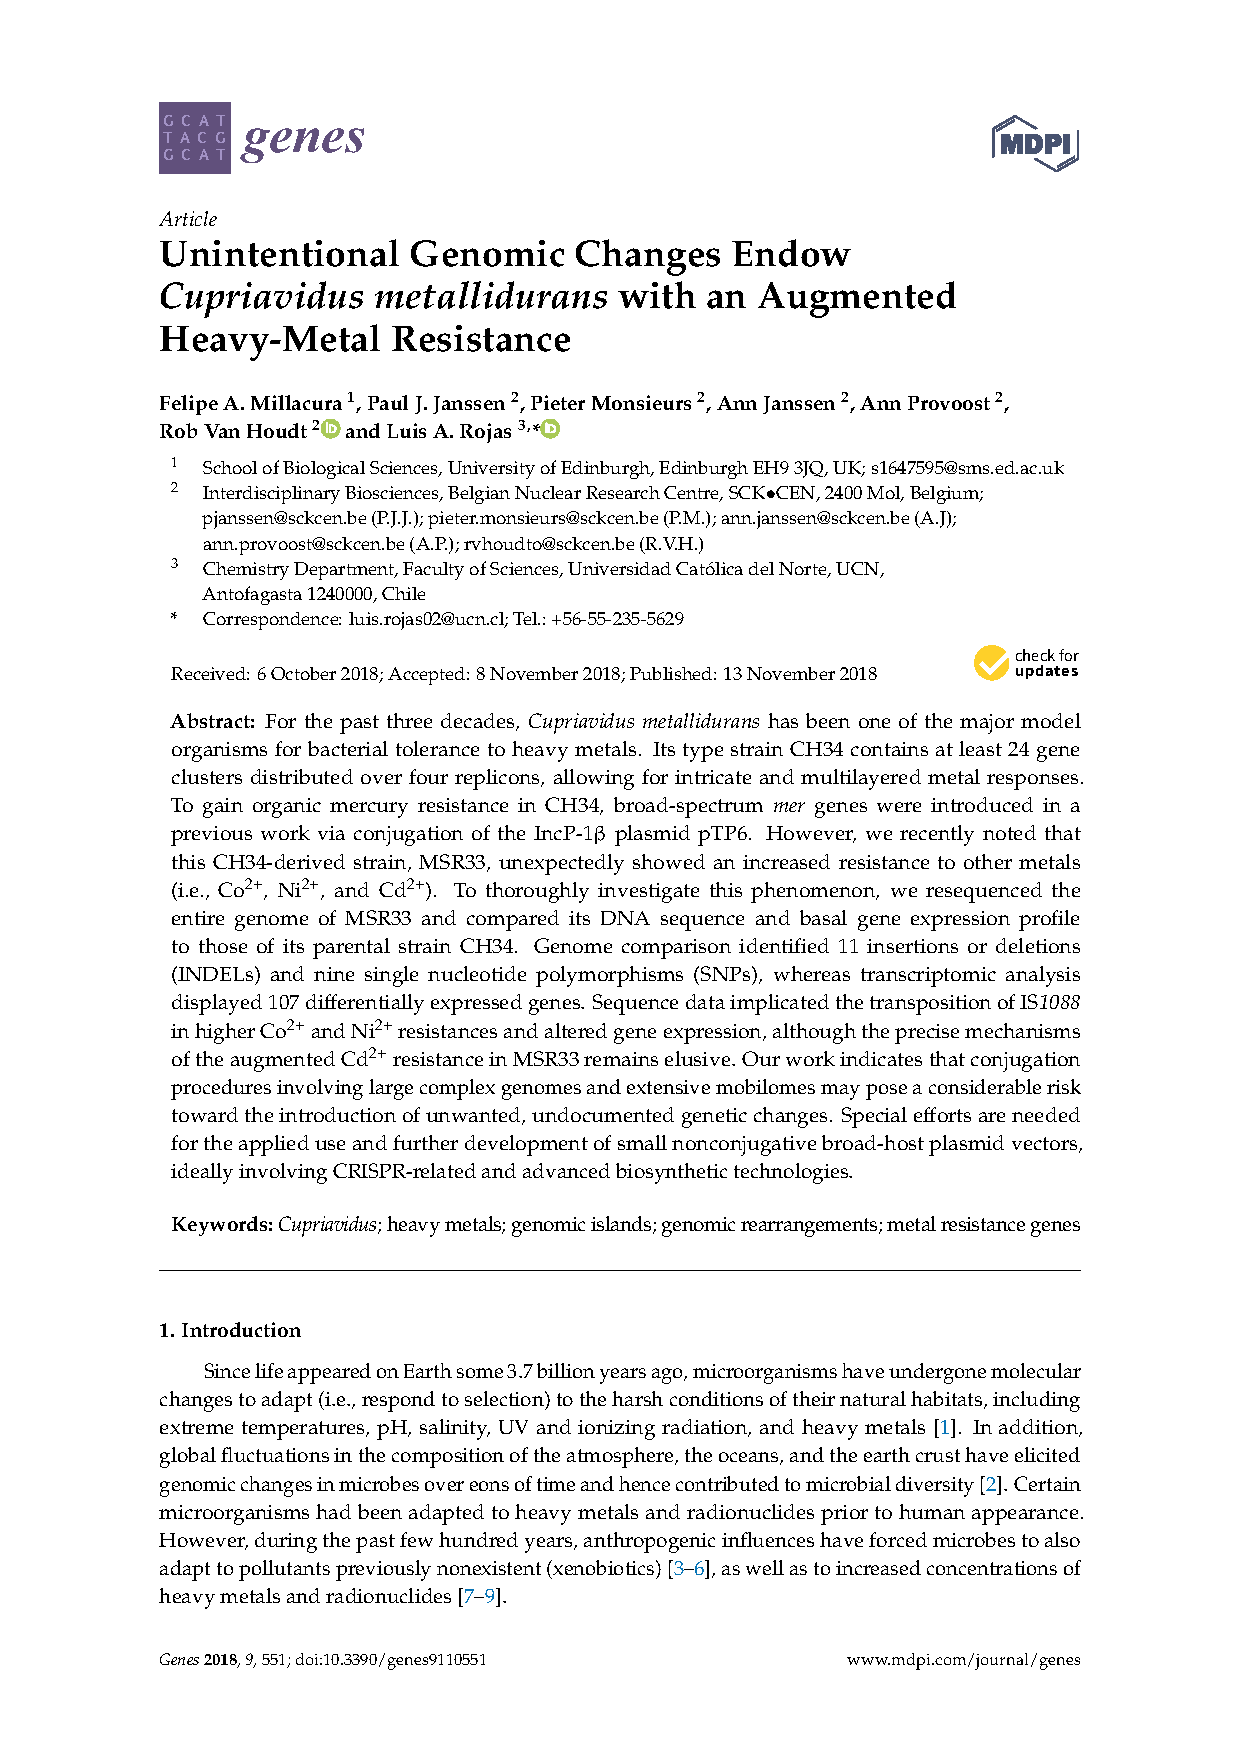
\includepdf[pages=-, width=\paperwidth,height=\paperheight, offset= 20 -20]
{\dir/genes-09-00551(1).pdf}



\end{document}
